\clearpage
\section{Sample selection}
\label{sec:Sample_selection}

\subsection{MUSE-GTO MAGIC}

MAGIC (MUSE-gAlaxy Groups In Cosmos) is  an ESO spectroscopic survey (PI: T. Contini) of intermediate redshift (0.25 < z <  0.85) groups and clusters performed over 4.5 years (Dec 2014 - May 2019) as part of the MUSE Guaranteed Time Observations (GTO). About 100h of MUSE observing time has been used to cover a sample of 15 groups/clusters selected primarily in the COSMOS area following the group catalogue of \shortcite{Knobel2009} and \shortcite{Knobel2012}. The main objective of this survey is to investigate the impact of environment on the evolution of galaxy properties (SFR, kinematics, metallicity, etc) at intermediate redshifts. 

\subsection{COSMOS field}

\begin{table}[htbp]

	\centering
	\hspace{50pt}

	\begin{tabular}{ccccccc}
	\hline
	Group & Ra\textsuperscript{2} & Dec\textsuperscript{3} & Exposure\textsuperscript{4}  & Average & Total nb. & Nb. field \\
	
	ID\textsuperscript{1} & J2000 (\degree) & J2000 (\degree) & (hr) & seeing\textsuperscript{5} (") & galaxies\textsuperscript{6} & galaxies\textsuperscript{7} \\	
	
	
	\hline
	CGr32 & $149.92194$ & $2.520972$ & $3 \times 4.35$ & $0.51$ - $0.58$ & $277$ & $113$ \\
	\hline
	CGr34\_d & $149.87766$ & $2.502331$ & $5.25$ & $0.63$ & $74$ & $46$ \\
	\hline
	CGr34\_bs & $149.87766$ & $2.502331$ & $4.75$ & $0.58$ & $74$ & $46$ \\
	\hline
	CGr30\_d & $150.144225$ & $2.065971$ & $9.75$ & $0.67$ & $124$ & $65$ \\
	\hline
	CGr30\_bs & $150.144225$ & $2.065971$ & $6.25$ & $0.57$ & $124$ & $65$ \\
	\hline
	CGr84 & $150.057219$ & $2.599744$ & $5.25$ & $0.59$ & $92$ & $51$ \\
	\hline
	CGr84-N & $150.05967$ & $2.61275$ & $1$ & $0.51$ & $81$ & $38$ \\
	\hline
	CGr114 & $149.994285$ & $2.258044$ & $2.2$ & $0.68$ & $64$ & $45$ \\
	\hline
	CGr79 & $149.820686$ & $1.821825$ & $4.35$ & $0.60$ & $65$ & $37$ \\
	\hline
	CGr28 & $150.218094$ & $1.812667$ & $1$ & $0.62$ & $49$ & $29$ \\
	\hline
	CGr26 & $150.492767$ & $2.069139$ & $1$ & $0.59$ & $46$ & $31$ \\
	\hline
	CGr61 & $149.728741$ & $1.915987$ & $1$ & $0.64$ & $43$ & $29$ \\
	\hline
	CGr51 & $149.982756$ & $1.801899$ & $1$ & $0.6-0.7$ & $44$ & $29$ \\
	\hline
	CGr23 & $149.790782$ & $2.162648$ & $1$ & $0.68$ & $51$ & $32$ \\
	\hline
	
	\end{tabular}
	
	\caption[Main characteristics of the MUSE observations in the COSMOS area.]{Main characteristics of the MUSE observations in the COSMOS area at the beginning of the internship. Groups ending with \_d correspond to deep observations (full stacked OBs) and with \_bs correspond to best-seeing observations (only OBs with a seeing below $\SI{0.7}{"}$). 1. COSMOS group number 2. Group centre's right ascension 3. Group centre's declination 4. Exposure time of MUSE observations 5. Spatial resolution (PSF $\rm{FWHM}$) measured in MUSE data and given for the observed [OII] wavelength corresponding to the group's average redshift. 6. Total number of detected galaxies within MUSE FoV 7. Number of field galaxies with a secure redshift $0.4 \leq z \leq 1.4$}
	\label{table:MUSEfieldsProp}
\end{table}

The goal of this analysis is to perform a joint study of the morphology and the kinematics of field galaxies at intermediate redshift in the COSMOS area \shortcite{Scoville2007} using respectively HST ACS images and MUSE data. To this end, a set of $12$ galaxy structures (groups or clusters) was selected. The COSMOS area was chosen because of the large number of multi-band photometric data available for the galaxies in this field and the presence of rich galaxy groups.\\

Guaranteed Time Observations centred on the groups were performed, from which 14 different MUSE Fields of View (FoV) were obtained. Each is composed of multiple Observation Blocks (OB) of $40-\SI{60}{min}$ each with the Position Angle (PA) of the instrument rotated by $\SI{90}{\degree}$ between consecutive exposures. Most of the groups enter into one MUSE FoV, except for CGr32. Since this group\footnote{which appeared to be a cluster following new redshift measurements using MUSE data.} is more extended than the others, three slightly overlapping FoVs were taken around it. A couple of groups were also split into \textit{deep} and \textit{best-seeing} observations, the former combining all the OBs regardless of the average seeing in each OB, when the latter only kept those with an average seeing lower than $\SI{0.7}{"}$. The main characteristics of the observed MUSE fields, including the position of their centre, the MUSE exposure time per FoV, the average spatial resolution (PSF $\rm{FWHM}$) measured in MUSE data, the total number of galaxies and the number of field galaxies are listed in Table\,\ref{table:MUSEfieldsProp}. \\

The structures the MUSE fields were centred upon were chosen from \shortciteA{Knobel2009}, \shortciteA{Knobel2012} catalogues. This ensured them to have both a large set of corresponding photometric data available from \shortciteA{laigle_cosmos2015_2016} catalogue and HST images with a much better resolution (\SI{0.03}{arcsec/px} for HST). A few galaxies in CGr30\_deep might have also been detected within the data cubes but not in HST images. This is because a blind source detection was performed with ORIGIN \shortcite{Bacon2017}, which can deblend sources even below the PSF, and identify galaxies (mostly at $z > 3$) not seen in broad-band HST images but which are easily detected with MUSE thanks to their bright emission line (mainly $\rm{Ly}\alpha$). In addition, there were also a few galaxies detected with MUSE in the vicinity of stars which were masked when creating \shortciteA{laigle_cosmos2015_2016} catalogue.

\subsection{Prior information on the galaxies}

\subsubsection{Galaxies in structures}

This internship was planned to be similar in many aspects to what  V. Abril-Melgarejo, a 2nd year PhD student supervised by B. Epinat at LAM, Marseille, is doing. She studies the morphology and the kinematics of galaxies within the structures observed with MUSE in the same fields as those we are using in this work. The main difference is that we are focusing on "field" galaxies when she only studies those in structures. To differentiate between group and field galaxies, a Friend of Friends algorithm (FoF) was run prior to my arrival on the galaxies in the MUSE fields. Thus, each galaxy was labelled either as belonging to a structure or as "field" galaxies. Additionally, a morphological analysis had already been performed by V. Abril-Melgarejo with GALFIT on galaxies in structures only. Two Sérsic profiles with fixed Sérsic indices ($n = 1, 4$) were used to model the light profile of these galaxies as a combination of a disk and a bulge component. Hence, their intensity can be written as

\begin{equation}
	I(r) = I_{e, \rm{d}} \, e^{-b_1 \left [ \frac{r}{R_{\rm{d}}} -1 \right ]} + I_{e , \rm{b}} e^{- b_4 \left [ \left ( \frac{r}{R_{\rm{b}}} \right )^{1/4} -1 \right ]}
	\label{eq:GALFIT_light_profile}
\end{equation}
where $I_{e, \rm{d}}$, $I_{e, \rm{b}}$ are the effective intensities of the disk and the bulge component respectively and $R_{\rm{d}}$, $R_{\rm{b}}$ their half-light radii. Therefore, we already have in hand morphological information for roughly half of the total sample including model parameters as described above, but also morphological parameters such as the ellipticity of the galaxies, the position angle of their kinematical main axis (which can be different from the morphological PA), and their size (half-light radius).

\subsubsection{Morphological information from COSMOS catalogues}

The total number of galaxies detected in the 16 MUSE fields in the COSMOS area is around $1000$. Roughly half of them belong to structures and the other half are labelled as "field" galaxies. However, not all of them are useful to our study. Some may be too close to the edge of the MUSE field-of-view, others may be too noisy with a low SNR, or even too small, preventing any relevant kinematical modelling. It is thus mandatory to apply a selection on our data set of field galaxies, first to save time for the analysis, but also to reduce uncertainties.\\

Our goal is to perform a joint study of the morphology and the kinematics of these galaxies. The tools and the models for the kinematical modelling were already developed as they were used by V. Abril-Melgajero. On the other hand, fitting morphological models with software such as GALFIT \shortcite{GALFIT} or SExtractor \shortcite{SExtractor} would have required additional time which we did not have during this internship. Hopefully for us, morphological modelling had already been performed on some galaxies in the COSMOS field, so we could focus on the kinematical part. \\

Morphological information can be found in various catalogues and tables\footnote{\url{https://irsa.ipac.caltech.edu/data/COSMOS/tables/morphology/}}. To start with, we decided to use the two most complete we could find, that of Tasca and Cassata. Both catalogues, which are not published but publicly available, contain morphological information including the central position of the galaxy, its half-light radius, concentration and asymmetry parameters, ellipticity, PA of the major morphological axis, and so forth for roughly $232 000$ galaxies found in the ACS catalogue from \shortciteA{Leauthaud2007}. The authors obtained morphological information either with a combination of SExtractor and Morpheus \shortcite{Abraham2007}, or with GIM2D \shortcite{GIM2D} using HST images. \\

Since we already had in hand a catalogue combining spectroscopic information (emission line fluxes, redshift, etc.) from MUSE measurements with photometric data from \shortciteA{laigle_cosmos2015_2016}, we cross-matched it with Cassata's and Tasca's tables to collect their morphological parameters. We cross-matched first with each catalogue separately, and then with both, using the right ascension $\alpha$ and declination $\delta$ of the centre of the galaxies, allowing for a maximum separation between the MUSE source and the closest source within the catalogues of $\SI{1}{arcsec}$. This procedure was done for structure galaxies as well in order to use them to check the robustness and consistency of the catalogues parameters.



\newpage
\subsection{Checking catalogues values consistency}
\subsubsection{Reasons for checking catalogues values consistency and robustness}

\begin{figure}[htbp]
	\centering
	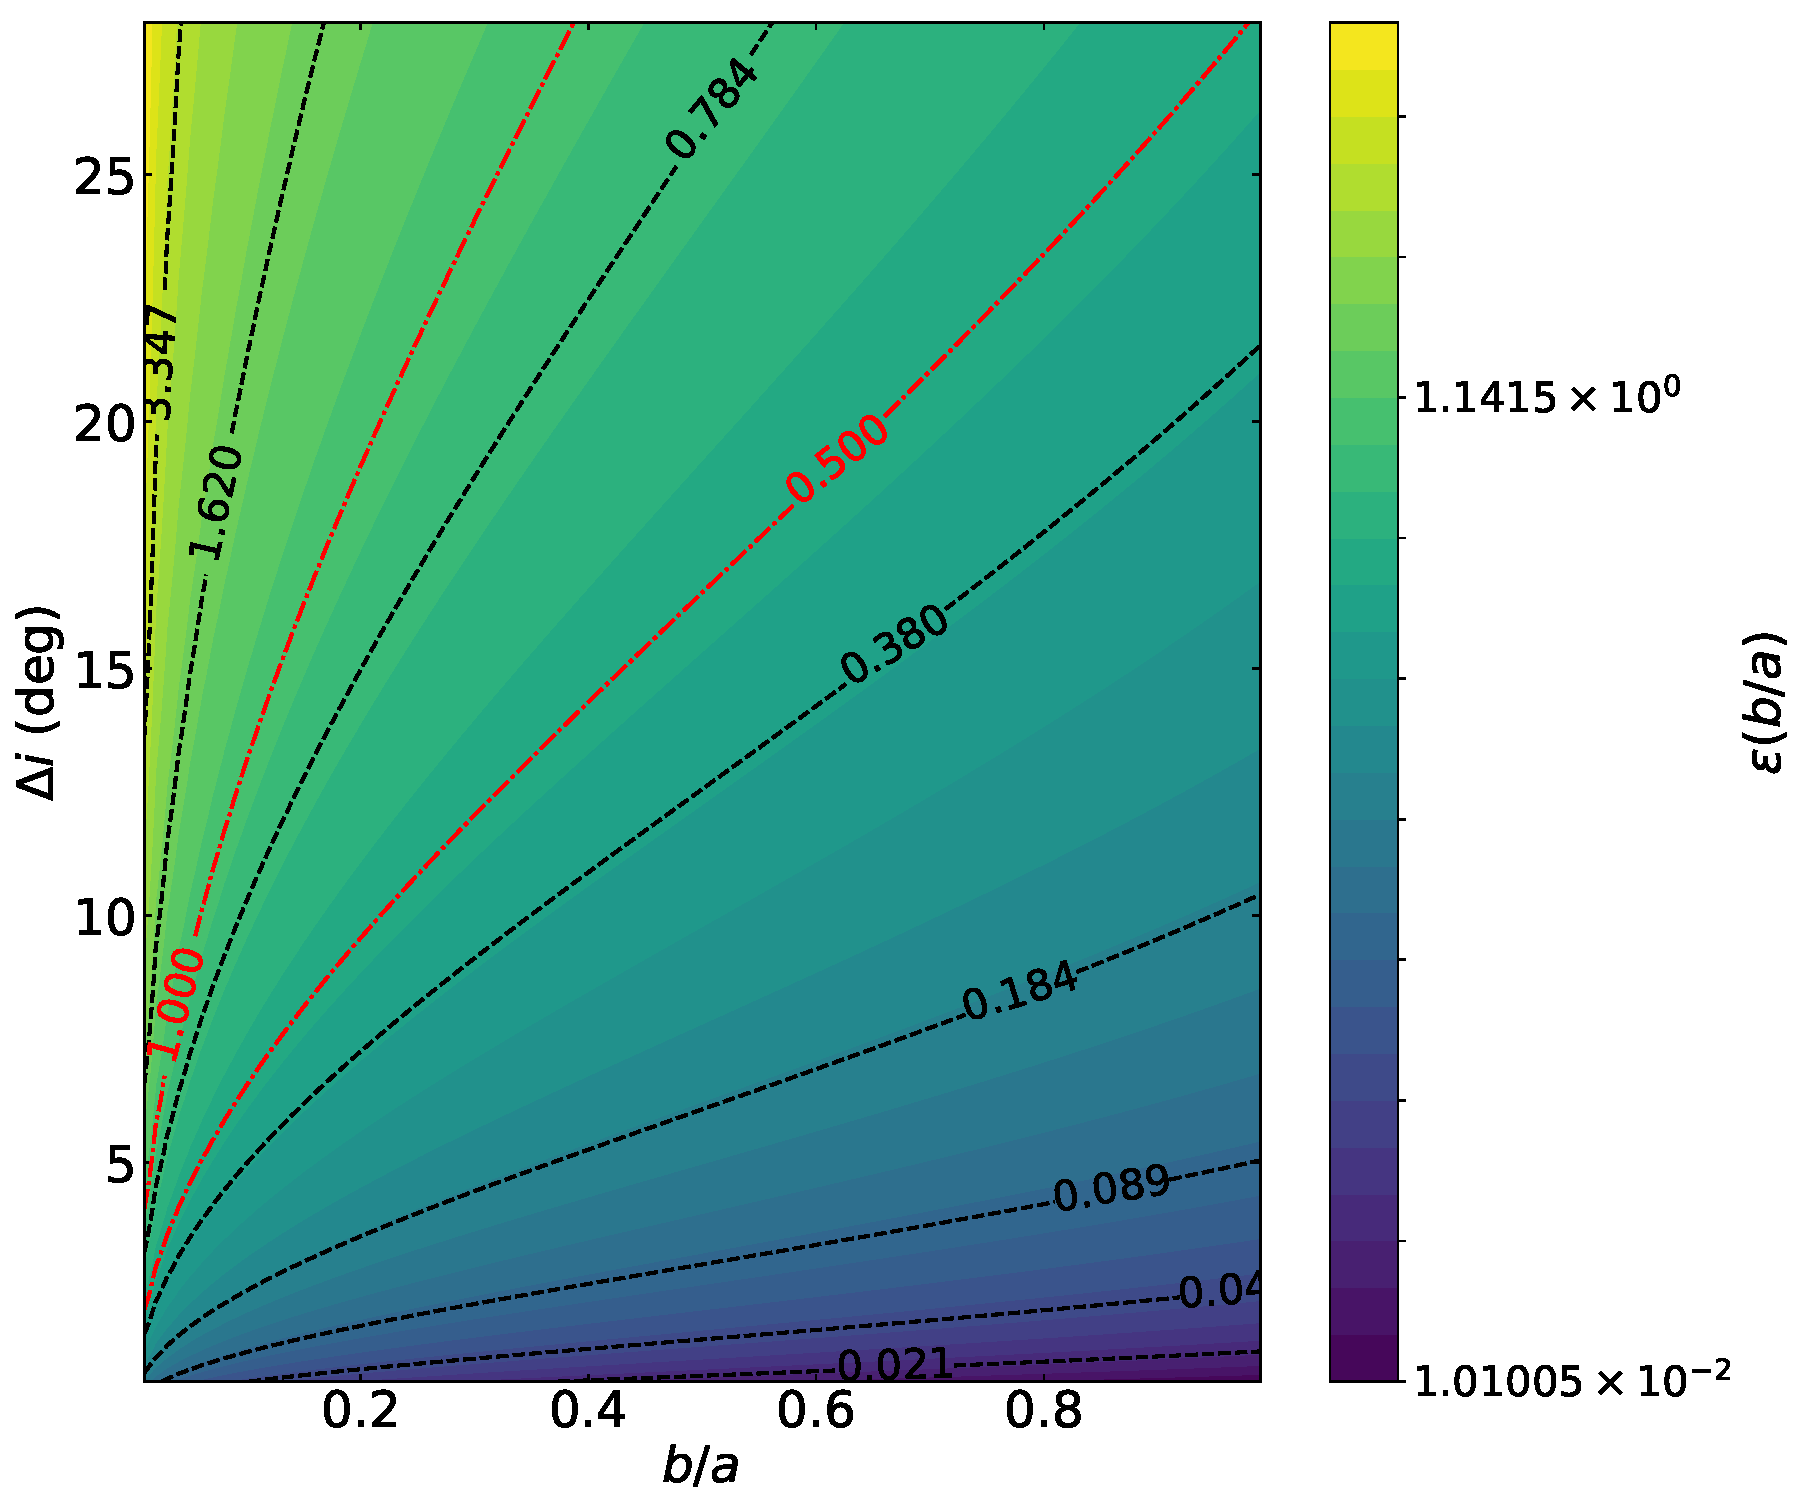
\includegraphics[width=\linewidth]{{../Plots/RelError_on_inc_versus_b_a}.pdf}
	\caption[Theoretical evolution of inclination uncertainty with $b/a$]{Theoretical uncertainty of the inclination as a function the minor-axis to major-axis ratio $b/a$ and its absolute (left) or relative (right) error. Contours are plotted in black dashed lines, with the red ones corresponding to a $50\%$ and $100\%$ error on $b/a$. The term error represents here any kind of uncertainty which could be used as an error estimate on $b/a$. This illustrates the importance to have measures of $b/a$ as reliable as possible for the kinematical modelling.}
	\label{fig:erreur_inclinaison}
\end{figure}

As a first step, we must select a sample based on relevant criteria. This is meant to ensure that we have reliable morphological and kinematical parameters and to reduce statistical errors. Given that any kinematical modelling relies on prior morphological information (galaxy centre, ellipticity, $\rm{PA}$), we can only use a combination of values derived from spectral fitting, for instance the [OII] $\rm{SNR}$, and from morphological modelling such as measures of radius and inclination to select our sample.  \\

Before this internship, spectral fitting on the integrated spectra of the galaxies had already been done, and we combined our data with morphological information from COSMOS catalogues as discussed in the previous section. Potentially useful morphological information included half-light radii, magnitudes, ratios of minor to major axis ($b/a$) or equivalently a measure of the ellipticity of the galaxies. Nevertheless, using this data without checking first how well it compares to values found in other catalogues and/or derived using different softwares/models could lead to high biases. Thus, before discussing any selection criteria for our sample, we must first assess the reliability of the parameters we are going to use in next sections. \\

Important values to check are the half-light radius, as it will be used to select our sample, the $b/a$ ratio and the $\rm{PA}$ since these are prior information for the kinematical modelling. We also checked if there was a correlation between the parameters obtained using the bulge/disk decomposition with GALFIT and the catalogues. The axes ratio has a crucial importance since it is directly related to the inclination of the galaxy on the sky through Eq.\,\ref{eq:inclinaison}. Given a certain error $\Delta (b/a)$, and using the variance formula to compute an uncertainty $\Delta f = | \partial_x f | \Delta x$ of a function $f$, we find for the inclination

\begin{equation}
	\Delta i = \Delta (b/a) \left | \frac{b}{a} \left ( 2 - \frac{b}{a} \right ) \right | ^{-1/2}
	\label{eq:error_inclination}
\end{equation}

This is illustrated in Fig.\,\ref{fig:erreur_inclinaison} where $\Delta i$ has been plotted as a function of $b/a$ and its error (absolute on the left, relative on the right). Contours of the error on $b/a$ have been over-plotted to show how evolves the uncertainty on $i$ given a fixed error on $b/a$. As expected, the higher the error on $b/a$ the higher the uncertainty on $i$. An error as high as 50\% could yield $\Delta i \approx \SI{27}{\degree}$, though this value is reached for $b/a \approx 1$ where the axes ratio is the least constrained by the morphology. Nevertheless, Eq.\,\ref{eq:error_inclination} is only a linear approximation and should not be used for too high values of $\Delta (b/a)$. A more appropriate error on $b/a$ of 20\% gives a maximum $\Delta i$ slightly above $\SI{10}{\degree}$, which is acceptable. Since the inclination has a strong impact on the galaxy intrinsic maximum rotational velocity, and potentially on the classification of galaxies as rotationally supported or dispersion dominated, this shows we must check carefully that the values of axes ratios are consistent between catalogues.

\subsubsection{Catalogues used for comparison}

We cross-matched our catalogue of galaxies detected by MUSE in COSMOS with Cassata's and Tasca's. However, as can be seen in Fig.\,\ref{fig:comp_radii_with_bulge_or_disk_radius} and \ref{fig:comp_radii}, we found large discrepancies between the parameters. Thus, to better understand their origin, we chose to cross-match our catalogue with another one (Zurich). This table has fewer HST counterparts of MUSE galaxies than in the other two but it contains additional morphological information which we can use for the comparison. In addition to that, we already had GALFIT morphological information on $\sim 500$ group galaxies with strong confidence in their value. Therefore, we chose to compare the data in the three morphological catalogues with that of GALFIT.

\subsubsection{Total magnitudes}
\label{sec:tot_mag}

\begin{figure}[htbp]
	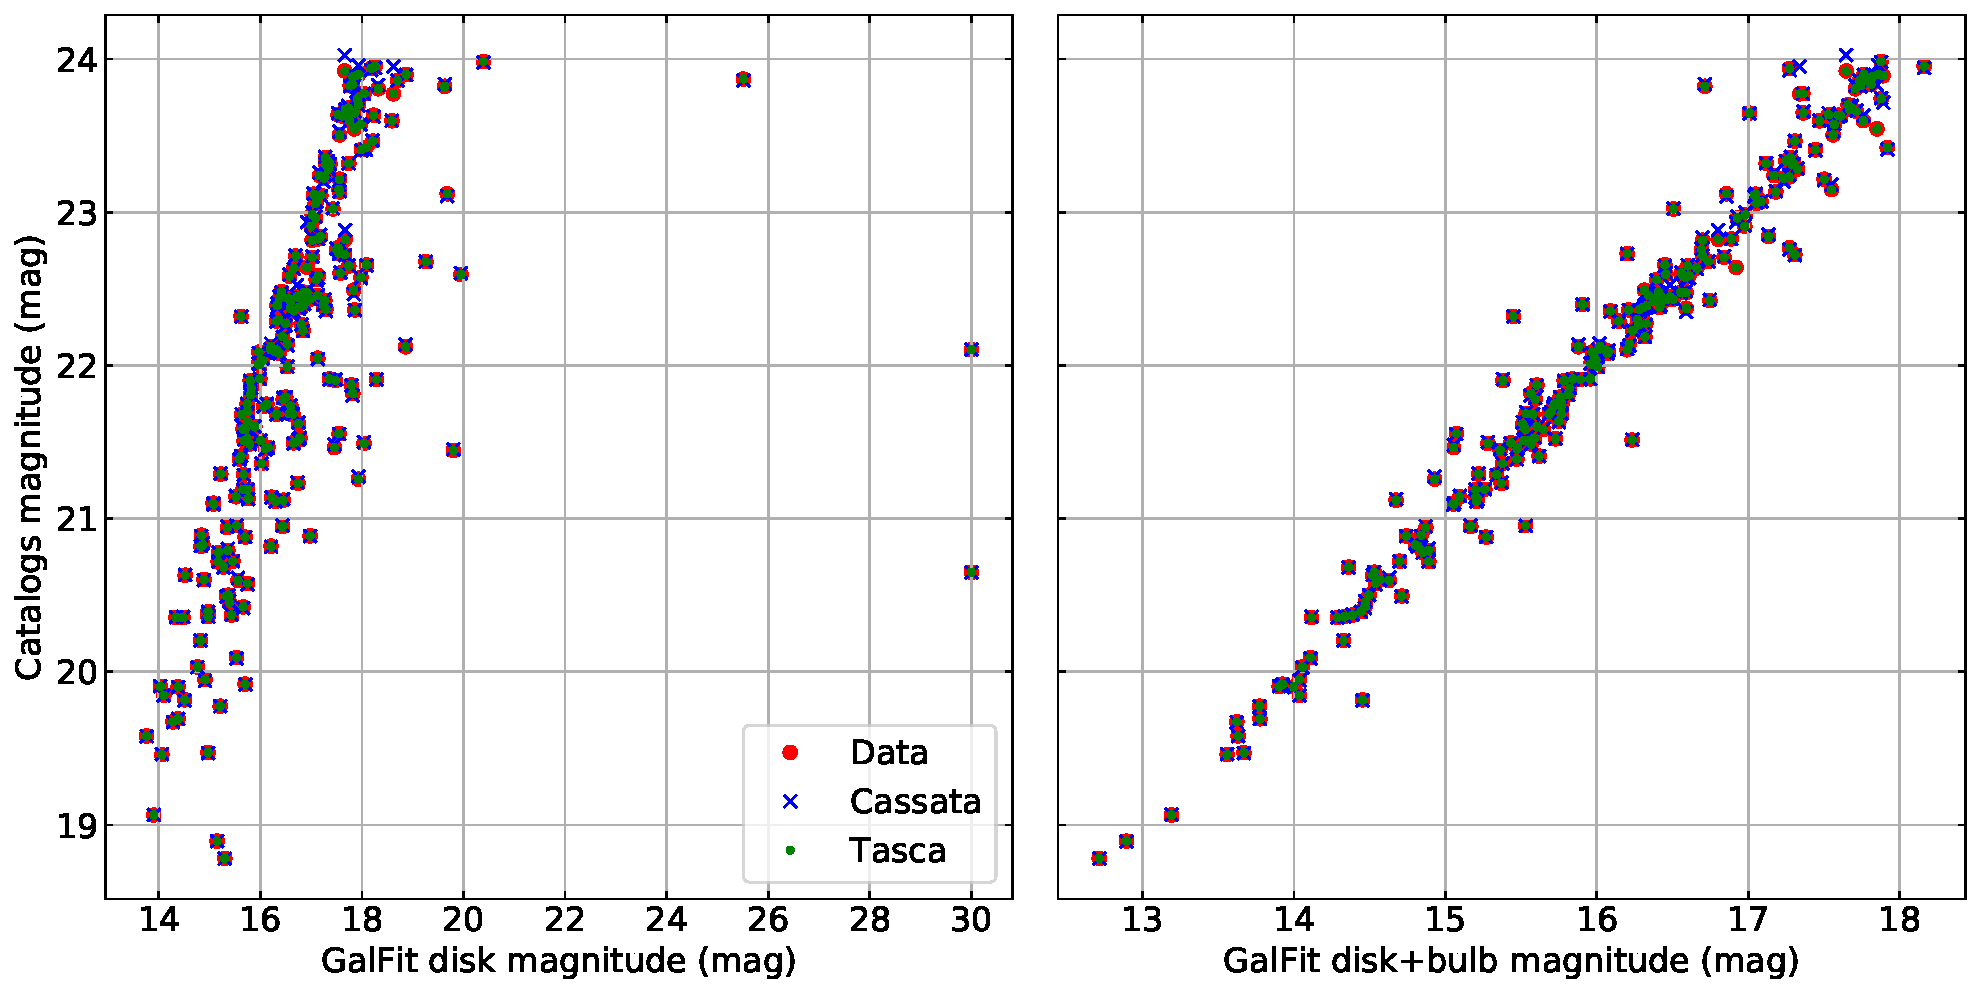
\includegraphics[width=\linewidth]{../Plots/catalogMag_against_GalfitMag_corrected.pdf}
	\caption[Comparison between GALFIT and catalogues magnitudes]{Comparison between the morphological catalogues magnitudes and that of GALFIT for cluster galaxies. Magnitudes from the catalogues agree well between each other. Left: compared with GALFIT disk magnitude only. The slope is too high and a few points are scattered far from the line. Right: compared with the total GALFIT magnitude as defined in Eq.\,\ref{eq:tot_mag_final_version}. The plain line represents the best-fit linear relation. We find a zero-point offset $(5.96 \pm 0.04)\, \rm{mag}$ (see Sec.\,\ref{sec:tot_mag}) and a scatter of about $\SI{0.2}{mag}$.}
	\label{fig:comp_mags}
\end{figure}

The first value we compared is the apparent magnitude. The three catalogues provide a measure of the total magnitude derived from fitting with a single Sérsic profile with a free Sérsic index $n$ on HST images. Given that V. Abril-Melgajero  modelled the group galaxies light profiles with GALFIT using two Sérsic profiles with fixed Sérsic indices ($n = 1, 4$), we have two measures of their magnitude: one for the bulge component $m_{\rm{b}}^{\rm{GF}}$, and another for the disk component $m_{\rm{d}}^{\rm{GF}}$. To have a meaningful comparison between magnitudes, we need to combine both to get the GALFIT total magnitude. Either component is defined as

\begin{equation}
	m_i^{GF} = -2.5 \log_{10} \left ( F_i^{\rm{GF}} \right ) + \rm{C}
	\label{eq:disk_bulge_lum}
\end{equation}
 where $i = \rm{b, d}$ represents either the bulge or the disk, $F = L/{4 \pi D^2}$ is the flux of the galaxy in some band, $L$ its intrinsic luminosity, $D$ its cosmological luminosity distance to us and $\rm{C}$ a constant which will depend on the band used. Considering that the two components have different luminosities but are located at the same distance, we can add the fluxes together. Thus the total GALFIT magnitude can also be written as

\begin{equation}
	m_{\rm{tot}}^{\rm{GF}} = - 2.5 \log_{10} \left ( F_{\rm{b}}^{\rm{GF}}  + F_{\rm{d}}^{\rm{GF}} \right ) + \rm{C}
	\label{eq:tot_mag}
\end{equation}

Inverting Eq.\,\ref{eq:disk_bulge_lum} to get the components flux as a function of their magnitude and inserting it into Eq.\,\ref{eq:tot_mag} yields

\begin{equation}
	m_{\rm{tot}}^{\rm{GF}} = -2.5 \log_{10} \left [ 10^{-\frac{m_{\rm{b}}}{2.5}} + 10^{-\frac{\rm{m_d}}{2.5}} \right ]
	\label{eq:tot_mag_final_version}
\end{equation}

This is the value that should be compared with the three catalogues magnitudes. Fig.\,\ref{fig:comp_mags} shows how these scale with each other and with GALFIT disk magnitude on the left, and the total magnitude from Eq.\,\ref{eq:tot_mag_final_version} on the right. As expected, the catalogues give the same value except for a few points. We see that the total GALFIT magnitude gives a much better, poorly scattered linear relation with the catalogues magnitudes. Even though there is an offset between GALFIT and the catalogues, this is due to using different conventions for the constant term in Eq.\,\ref{eq:disk_bulge_lum}.

The same comparison was done on field galaxies, except we did not have GALFIT magnitudes in this case. We also found a good agreement between the catalogues magnitudes.






\newpage
\subsubsection{Morphological type classification}
\label{subsubsec:classification}

\begin{wrapfigure}{r}{.6\linewidth}
	\centering
	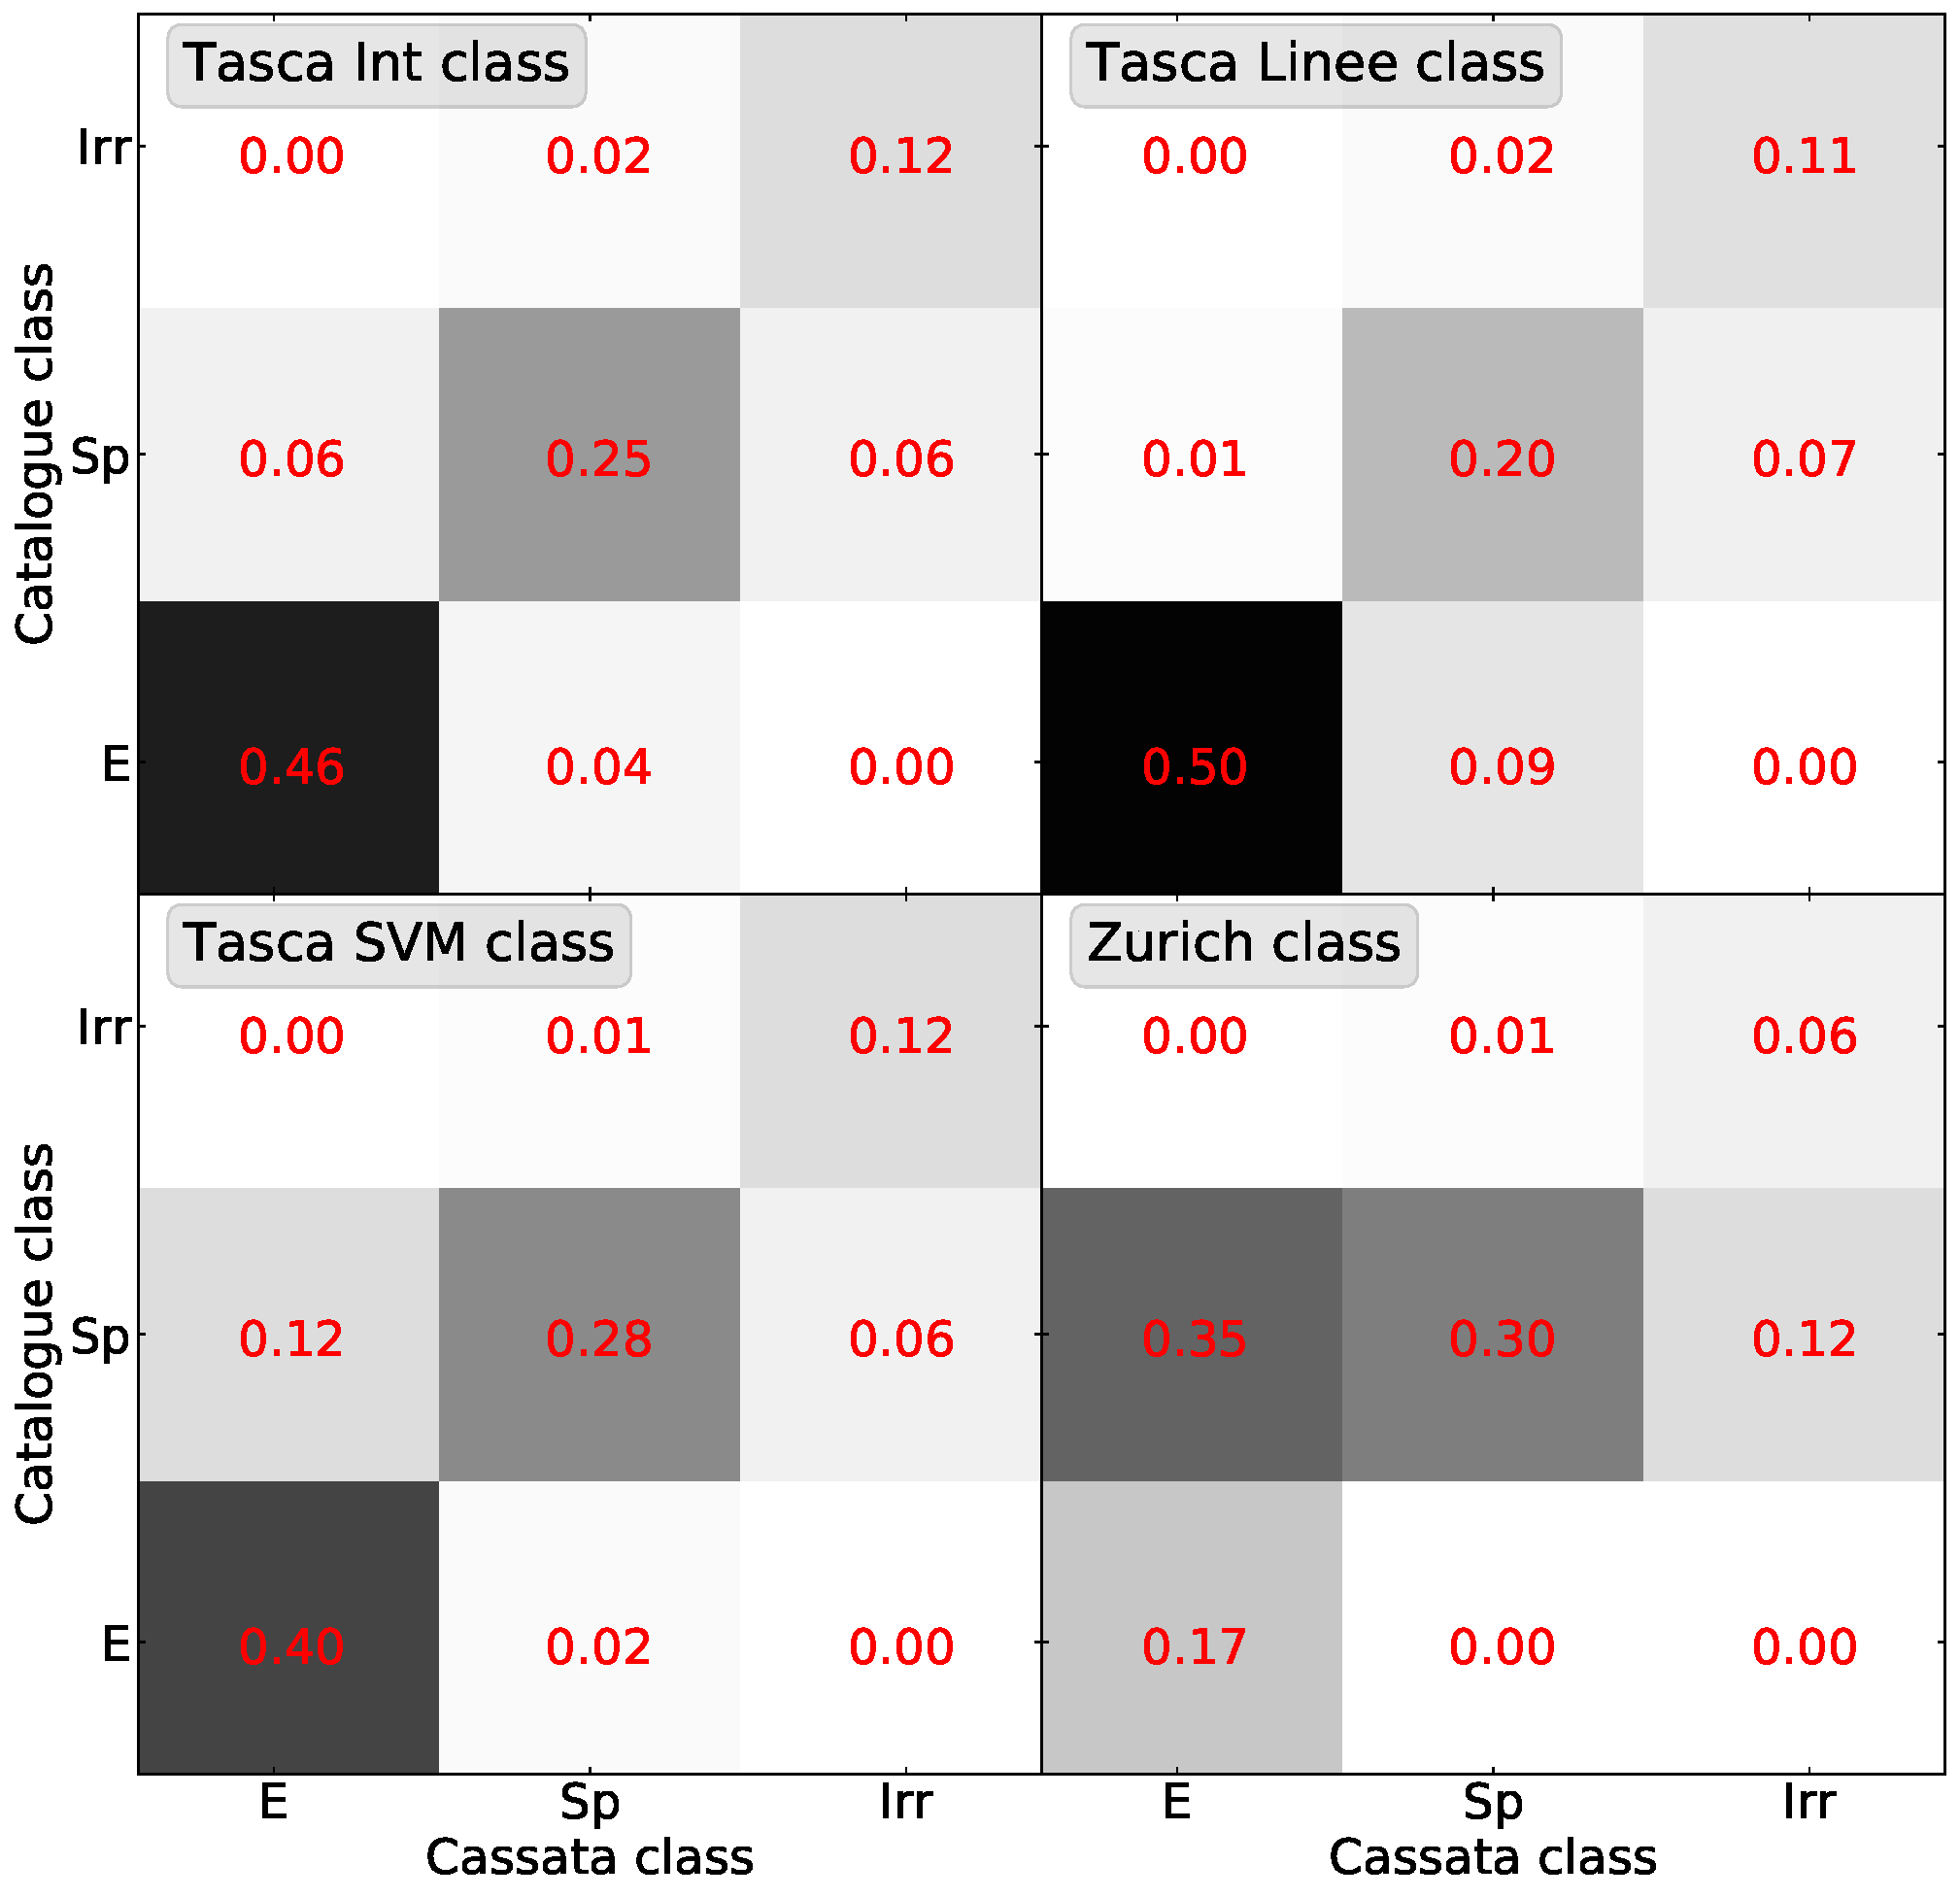
\includegraphics[width=\linewidth]{{../Plots/comparisonClassTypes}.pdf}
	\caption[Morphological types consistency]{Comparison between morphological types given in Tasca and Zurich catalogues against that of Cassata. Galaxies are labelled as follows: E for ellipticals, Sp for spirals/disks-like, Irr for irregulars. The percentage of galaxies falling into the given classes is indicated in red and the method compared with Cassata's is shown on the top left corner of each plot. We find good agreement between Tasca and Cassata types but not between Cassata and Zurich.}
	\label{fig:morpho_comp}
\end{wrapfigure}

We expect to have some discrepancies in our data because of the models used between GALFIT and SExtractor/GIM2D. To check this effect, we can study how the differences between morphological parameters scale with the morphological type of the galaxies. \\

For instance, if we use the disk half-light radius of GALFIT to compare with that of SExtractor, we might expect to have some scatter in our relation for the elliptical galaxies as the disk component is not the best one to describe them.\\

We used the classification given in the three morphological catalogues which are based on different methods. We provide below a short introduction to these classifications:\\


\begin{itemize}
	\item Cassata's catalogue gives a classification based on their morphological parameters. They use a set of $500$ reference galaxies with known parameters which they visually classify either as elliptical, disk-like/spiral or irregular. From this set, each time a new galaxy must be classified, its $11$ closest neighbours in parameter space are inspected and the most frequent class among them is assigned to the new galaxy.
	
	\item Tasca's catalogue gives different classifications based on three methods. The first is similar to the one used by Cassata. The second one uses the technique described in \shortciteA{Abraham1996b} using the asymmetry and concentration parameters. The last one uses a support vector machine to classify the galaxies.
	
	\item Zurich's catalogue gives a single classification called Zurich Estimator of Structural Type (ZEST) which is described in \shortciteA{Scarlata2007}. This method is based on a Principal Component Analysis (PCA). They only keep the first three Principal Components (PA) which retain most of the information present in the original five parameters (concentration, asymmetry, Gini coefficient, second-order moment of the brightest pixels producing $20\%$ of the total flux and the ellipticity of the galaxy).
\end{itemize}


\begin{wrapfigure}{r}{0.6\linewidth}
	\centering
	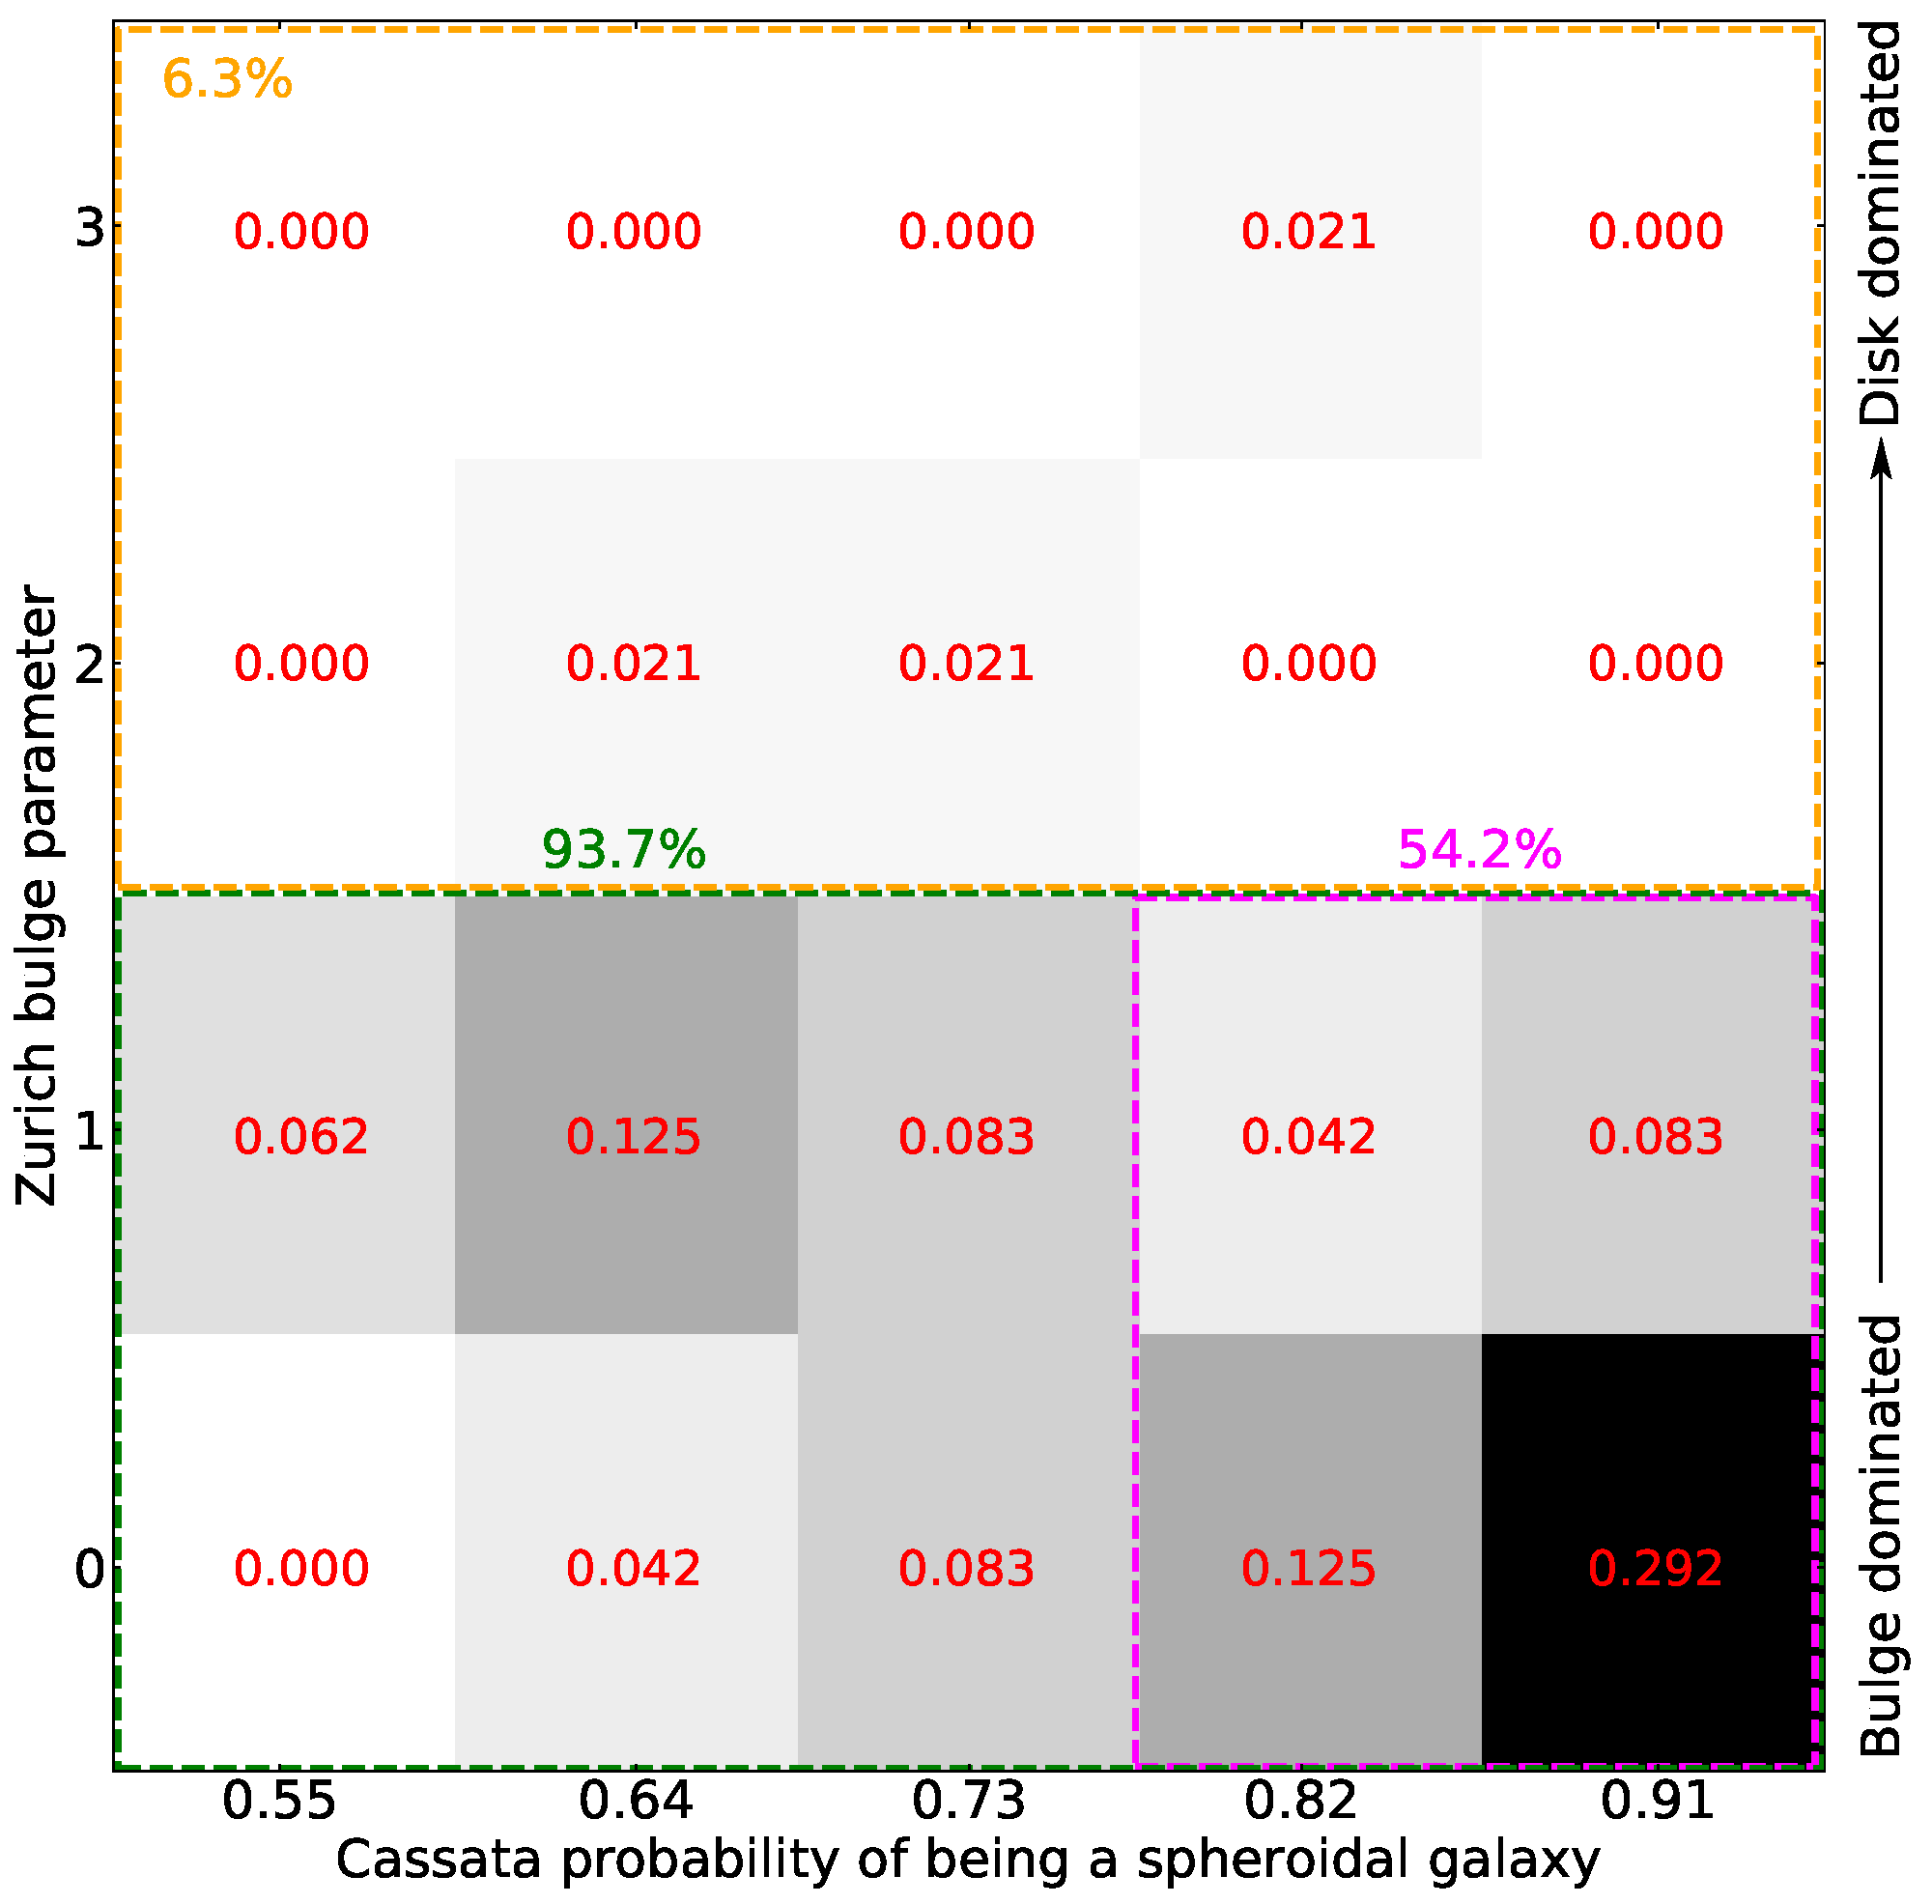
\includegraphics[width=\linewidth]{{../Plots/comparisonClassTypes_forWrongSpiralsOnly}.pdf}
	\caption[Origin of the classification discrepancy]{Comparison between Zurich's bulgeness parameter and Cassata probability that the galaxy belongs to the right classification for spheroidal galaxies (according to Cassata) misclassified as disk-like by Zurich. A low bulgeness value corresponds to a bulge dominated galaxy. We find that more than $93\%$ of galaxies are found to be bulge dominated according to Zurich. Around half of the discrepancy represented in Fig.\,\ref{fig:morpho_comp} corresponds to highly probable spheroidal galaxies classified by Zurich as disk-like with a dominant bulge.}
	\label{fig:bulge_against_prob}
\end{wrapfigure}

The morphological types given in Tasca's and Zurich's catalogues are compared against the class given by Cassata in Fig.\,\ref{fig:morpho_comp}. We observe a good agreement between Cassata's and Tasca's types with just a few elliptical galaxies labelled as disk-like and vice versa. Roughly $50\%$ of the galaxies appear to be elliptical. On the contrary, Zurich's classification seems to label more than $70\%$ of the galaxies as disk-like, including a large number of elliptical galaxies .\\

This effect can be better understood by comparing two additional information given in Cassata's and Zurich's catalogues. 
\begin{enumerate*}[label=(\alph*)]
	\item the probability, computed by Cassata, that the given classification is correct. This probability is computed as the number of galaxies within the $11$ closest neighbours with the given classification over $11$, and it can therefore vary between around $33\%$ and $100\%$.
	\item Zurich's bulgeness parameter which labels disk galaxies from bulge ($0$) to disk dominated ($3$).
\end{enumerate*} \\

This comparison is performed in Fig.\,\ref{fig:bulge_against_prob} for the galaxies classified as spheroidal by Cassata, but as disk-like by Zurich. We find that around half of the discrepancy in the classification comes from galaxies with a high probability of being disk-like in Cassata's, but with a dominant bulge in Zurich's. Moreover, if we do not take into account the probability given by Cassata, more than $90\%$ of these galaxies actually have a dominant bulge according to Zurich. Thus, it seems that most of the discrepancy we observe for this population of galaxies in terms of morphological classification is actually due to using different a different vocabulary. Cassata labels them as spheroidal because their light profile is dominated by the bulge component, but Zurich does make the distinction between spheroidal galaxies and disk-like with a dominating bulge.\\

Considering the aforementioned explanation of the observed discrepancy, and since we find a good agreement between Cassata's morphological type and those given by Tasca, we decided to use and to stick to Cassata's class throughout this work whenever we needed to separate galaxies between elliptical/disk-like/irregulars. This choice also ensured us to have the largest sample possible with a coherent classification as Cassata's catalogue is the one with the largest number of HST counterparts of MUSE galaxies in the COSMOS field.






\newpage
\subsubsection{Half-light radii}
\label{sec:comp_radii}

Perhaps the most important parameter we have to check is the half-light radius. Indeed, if we underestimate it, we might remove from our sample galaxies which are spatially resolved in MUSE data and therefore reduce our statistics. On the other hand, overestimating it would give us too many unresolved galaxies for which we would spend time removing noise dominated pixels without being able to perform their kinematical analysis in the end. Hence, it is mandatory to thoroughly check the values of the half-light radius from the three catalogues against that of GALFIT, and understand the origin of any discrepancies if there happens to be some. \\

We found a quite large disagreement between GALFIT half-light radii and those given in the morphological catalogues, as well as between them. This is illustrated in Fig.\,\ref{fig:comp_radii_with_bulge_or_disk_radius} and \ref{fig:comp_radii} where half-light radii in the catalogues are compared against that of GALFIT. Galaxies are colour coded according to the classification given in Cassata's catalogue. We checked that using Tasca's classifications as described in Sec.\,\ref{subsubsec:classification} did not change our conclusions. In these plots, we decided to use for the x-axis the half-light radius of the GALFIT disk component $R_{1/2 , \rm{d}}^{\rm{GF}}$ for all the galaxies, even though we might expect the ellipticals to be better described by their GALFIT bulge half-light radius. This choice is further discussed below.\\



The catalogues radii seem to be overestimated with respect to that of GALFIT for low $R_{1/2 , \rm{d}}^{\rm{GF}}$. Those compared in Fig.\,\ref{fig:comp_radii_with_bulge_or_disk_radius} and \ref{fig:comp_radii} are all derived from SExtractor and, given that it does not take into account the PSF in its fitting routine, we expect the PSF to dominate for galaxies with small angular sizes. On the contrary, GALFIT does take into account the PSF in its calculation, and therefore we expect its half-light radius to decrease with lower values of $R_{1/2 , \rm{d}}^{\rm{GF}}$. When focussing on galaxies with a GALFIT radius larger than the HST-ACS PSF $\rm{FWHM}$ which is around $\SI{0.15}{"}$ ($4 - \SI{5}{px}$), we observe a global underestimation for all the catalogues, up to roughly 50\%. This scatter is mainly due to elliptical galaxies. On the contrary, radii of disk-like galaxies have the least scatter and biais, especially the values given in Zurich's catalogue. This different behaviour between elliptical and disk-like galaxies might be explained, as mentioned above, by the fact that we are using the half-light radius of GALFIT disk component to asses the reliability of the elliptical galaxies radii given in the catalogues. A better choice may be to use the bulge component, which better describes the light profile of an elliptical galaxy, and its half-light radius for this population.\\

\begin{figure}[htbp]
	\centering
	\includegraphics[width=\linewidth]{{../Plots/plotsWithColourCoding/relErr_against_galFit1.5LightRadius_colourCoded_matchAllTypes_TwoGalFitRadii}.pdf}
	\caption[Radii comparison between catalogues and GALFIT using bulb and disk]{Relative error on the half-light radius between the catalogues and GALFIT. Points have been colour coded according to their classification given in Cassata's catalogue (Irr for irregular, Sp for disk-like, E for spheroidal). Top: GALFIT disk radius is used for all the points. We observe an underestimation of the catalogues radius with respect to that of GALFIT for elliptical galaxies. Bottom: same plot with GALFIT bulge radius used for elliptical galaxies. In this case, we find an overestimation of the radius.}
	\label{fig:comp_radii_with_bulge_or_disk_radius}
\end{figure}

\begin{figure}[htbp]
	\centering
	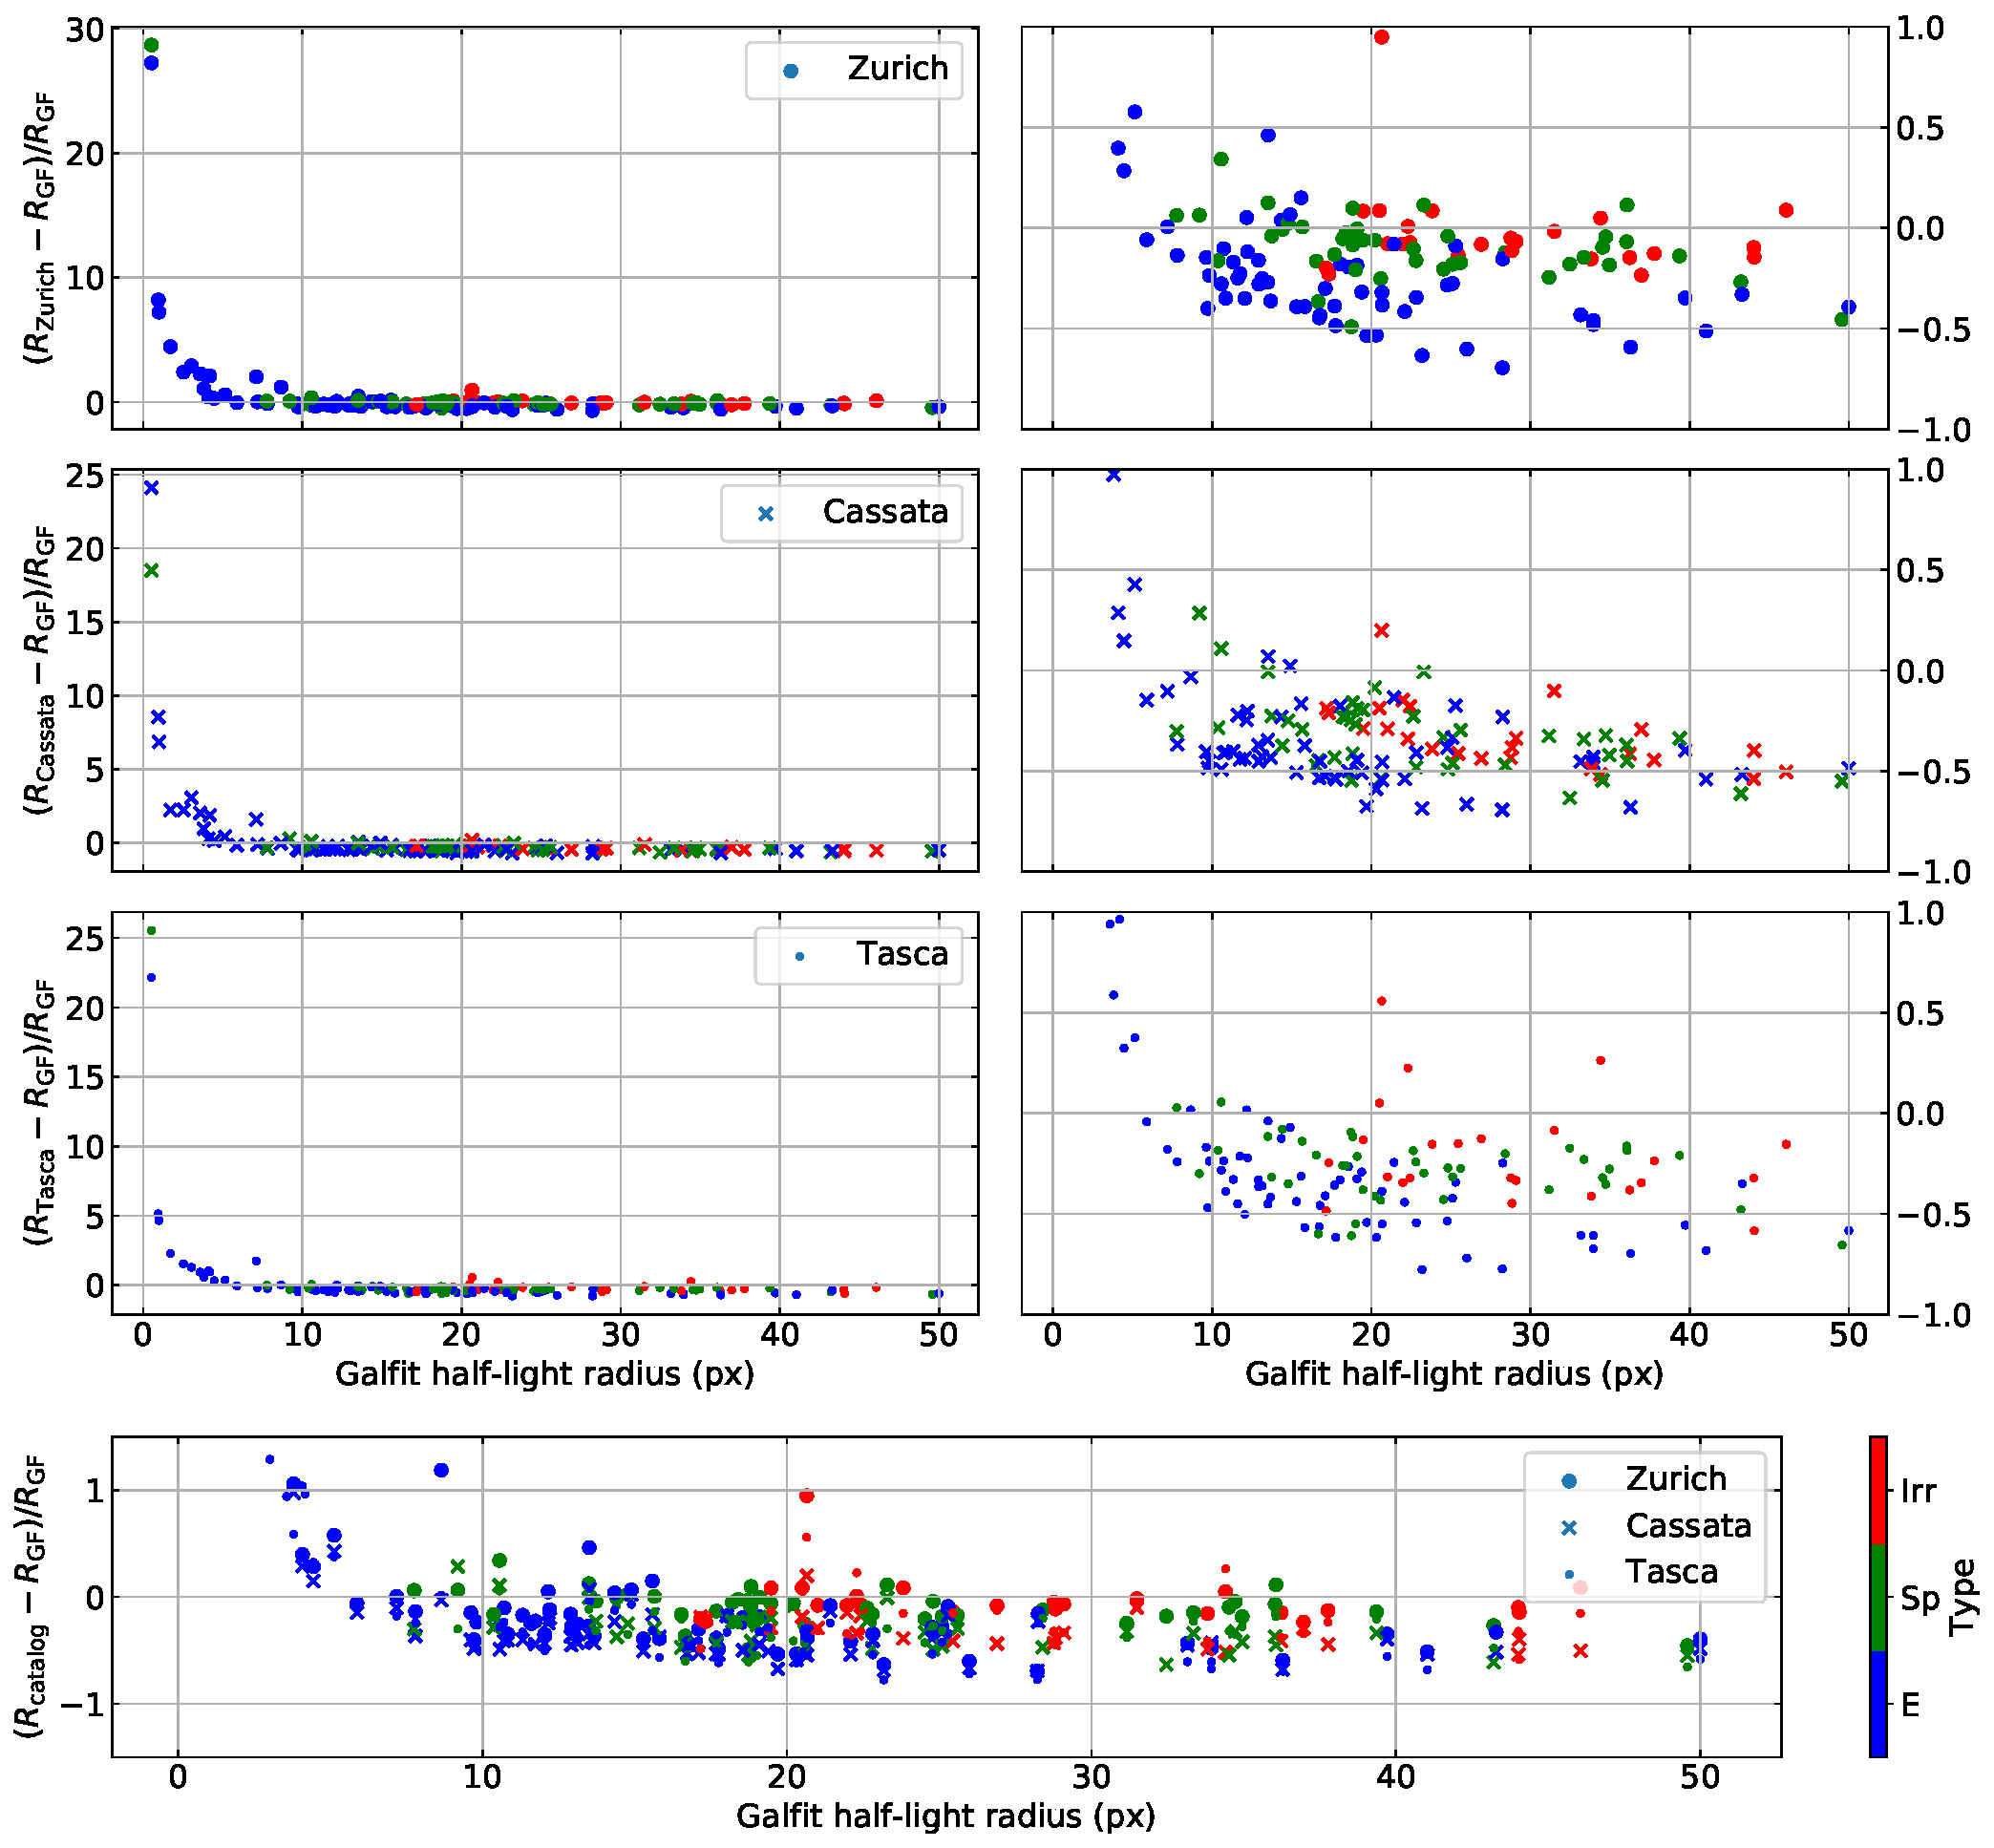
\includegraphics[width=\linewidth]{{../Plots/plotsWithColourCoding/relErr_against_GalFit1.5LightRadius_colourCoded_CassataType}.pdf}
	\caption[Radii comparison per catalogue]{Comparison between half-light radii from the morphological catalogues and the radius of GALFIT disk component. This plot is similar to Fig.\,\ref{fig:comp_radii_with_bulge_or_disk_radius} top plot but each catalogue was separated in its own subplot. Left: full range of relative error. Right: a zoom on the points with $R_{1/2}^{\rm{GF}} \geq \SI{5}{px}$.}
	\label{fig:comp_radii}
\end{figure}

If we split the galaxies into two categories, ellipticals and disks/irregulars, and if we use for the first category the bulge radius $R_{1/2 , \rm{b}}^{\rm{GF}}$, and for the second $R_{1/2 , \rm{d}}^{\rm{GF}}$, we find that elliptical galaxies half-light radii from the catalogues are now underestimated with GALFIT as shown in Fig.\,\ref{fig:comp_radii_with_bulge_or_disk_radius} lower plot. These results suggest that elliptical galaxies in this sample are neither dominated (in terms of radius) by the disk component, nor by the bulge in the GALFIT model. Even though we did not push further the analysis on this discrepancy, we still mention that the next step should be to directly compute the half-light radius of the GALFIT model by integrating Eq.\,\ref{eq:GALFIT_light_profile} up to half its total luminosity.


\begin{figure}[htbp]
	\centering
	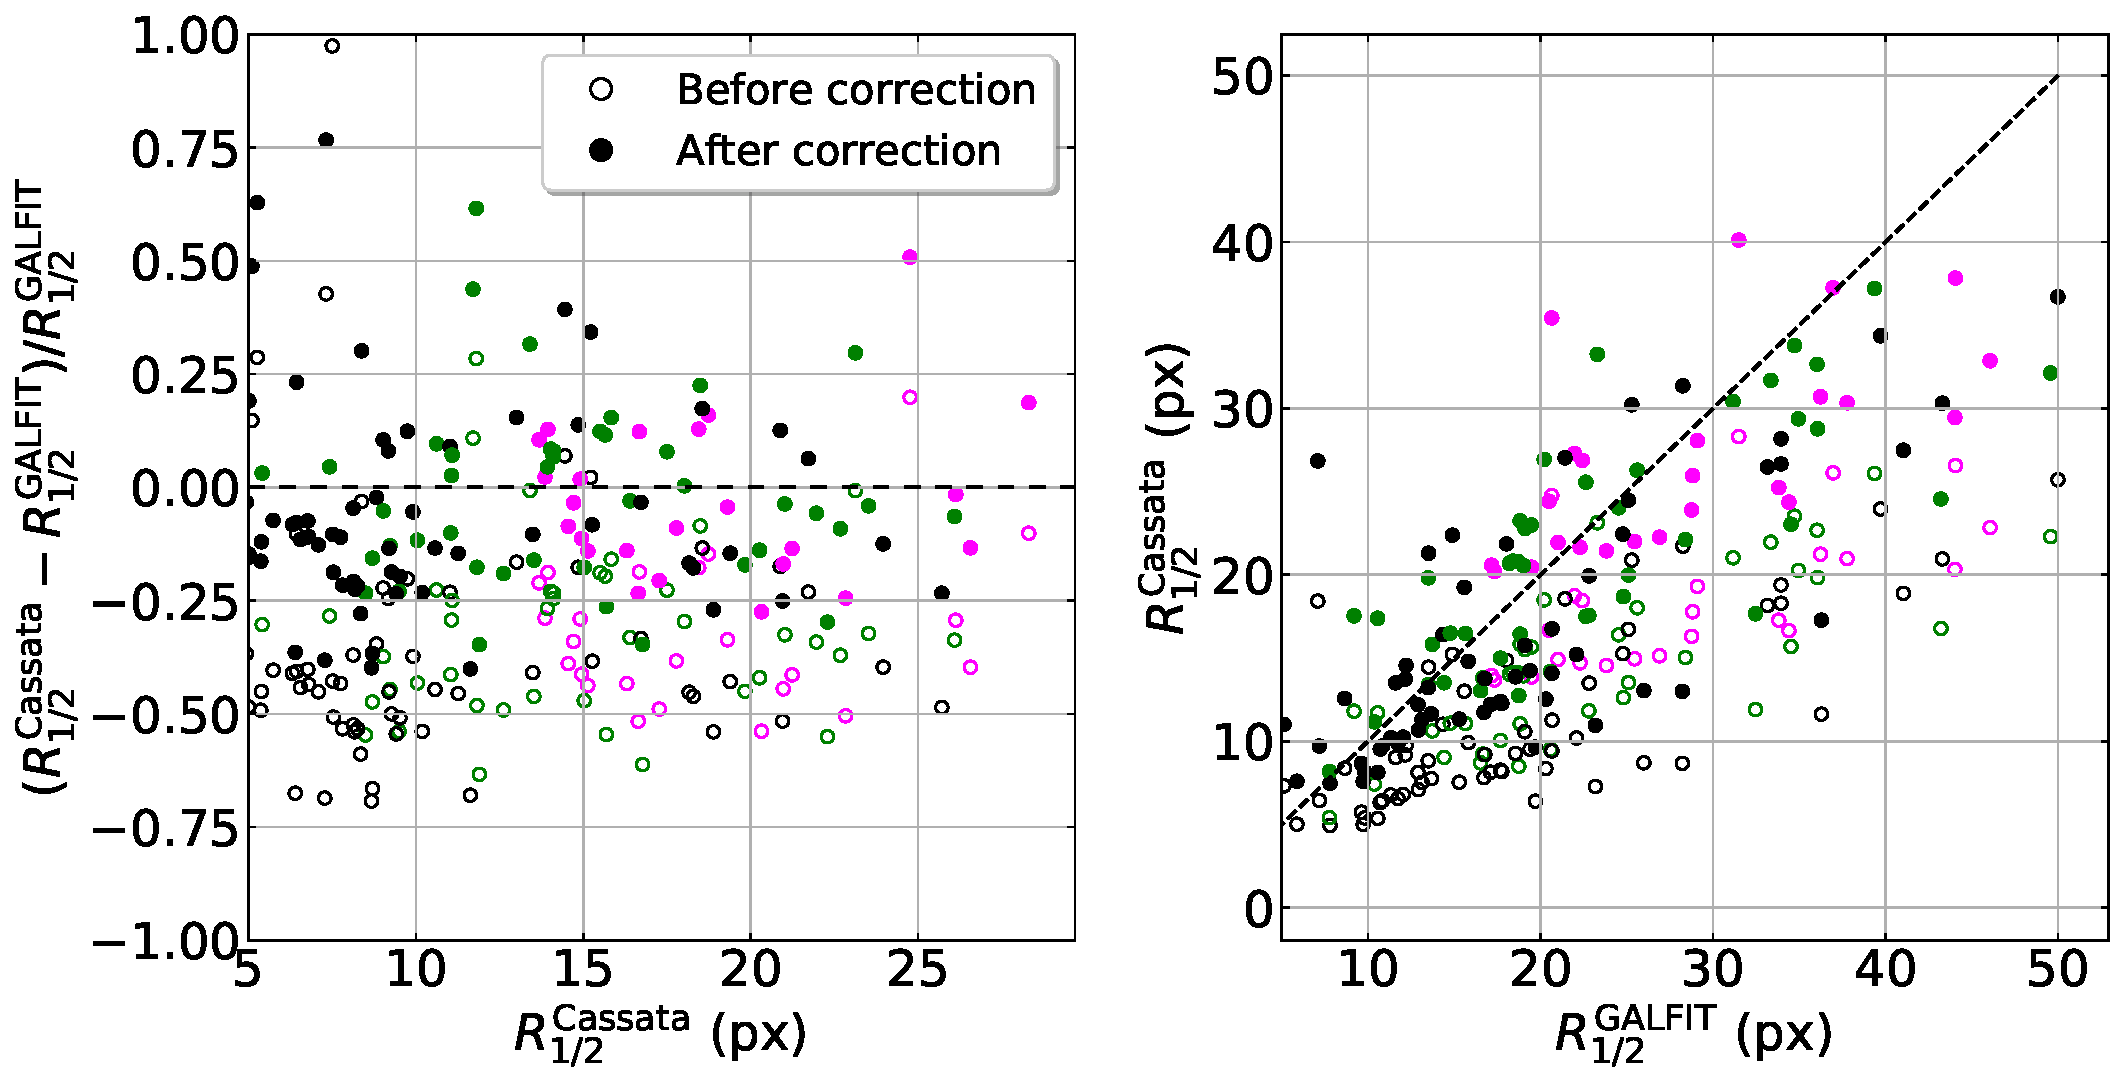
\includegraphics[width=\linewidth]{{../Plots/Selection_plots/correctedRadiusLinearRegression}.pdf}
	\caption[Half-light radius bias before/after correction]{Biais and scatter before and after applying the correction mentioned in the paragraph. The dashed line represents the 1-1 line if there was no bias. Left: half-light radius relative error as a function of Cassata's radius. Right: scaling between Cassata's and GALFIT radii. The scatter around $\SI{0.2}{px}$ is not significantly changed after the bias correction.}
	\label{fig:correction_biais_radius}
\end{figure}

Based on Fig.\,\ref{fig:comp_radii}, we decided to use the galaxies half-light radii given in Zurich catalogue, keeping in mind that we might have a non-negligible fraction of elliptical galaxies for which their value may be underestimated. However, this is the catalogue with least HST counterparts. Thus, in order to increase our sample, we also chose to select additional galaxies found in Cassata's catalogue but not in Zurich's. As it seems that Cassata's radius is more bias than Zurich's, we fitted a linear relation onto the relative error data, which translates as

\begin{equation}
	R_{1/2}^{\rm{Corrected}} = R_{1/2}^{\rm{Cassata}} \left ( 1 + \beta + \alpha R_{1/2}^{\rm{Cassata}} \right ) ^{-1}
\end{equation}
where $R_{1/2}^{\rm{Corrected}}$ is the new half-light radius after the bias correction and $\alpha$, $\beta$ the parameters of our fit. Based on previous arguments, we only fitted galaxies for which $R_{1/2}^{\rm{GF}} > \SI{5}{px}$. Once a best fit solution was found, we slightly adjusted it by applying a weight on ellipticals in order to limit their impact on disk-like galaxies radii which appeared to be too much overestimated without. We find $\alpha = 1.95 \times 10^{-3}$ and $\beta = -0.349$, which gives us $261$ field galaxies. We kept Zurich radius whenever a galaxy had one, and the bias corrected Cassata radius when we only had this value.





\newpage
\subsubsection{Ellipticity}

\begin{figure}[H]
	\centering
	\begin{minipage}[c]{0.49\linewidth}
		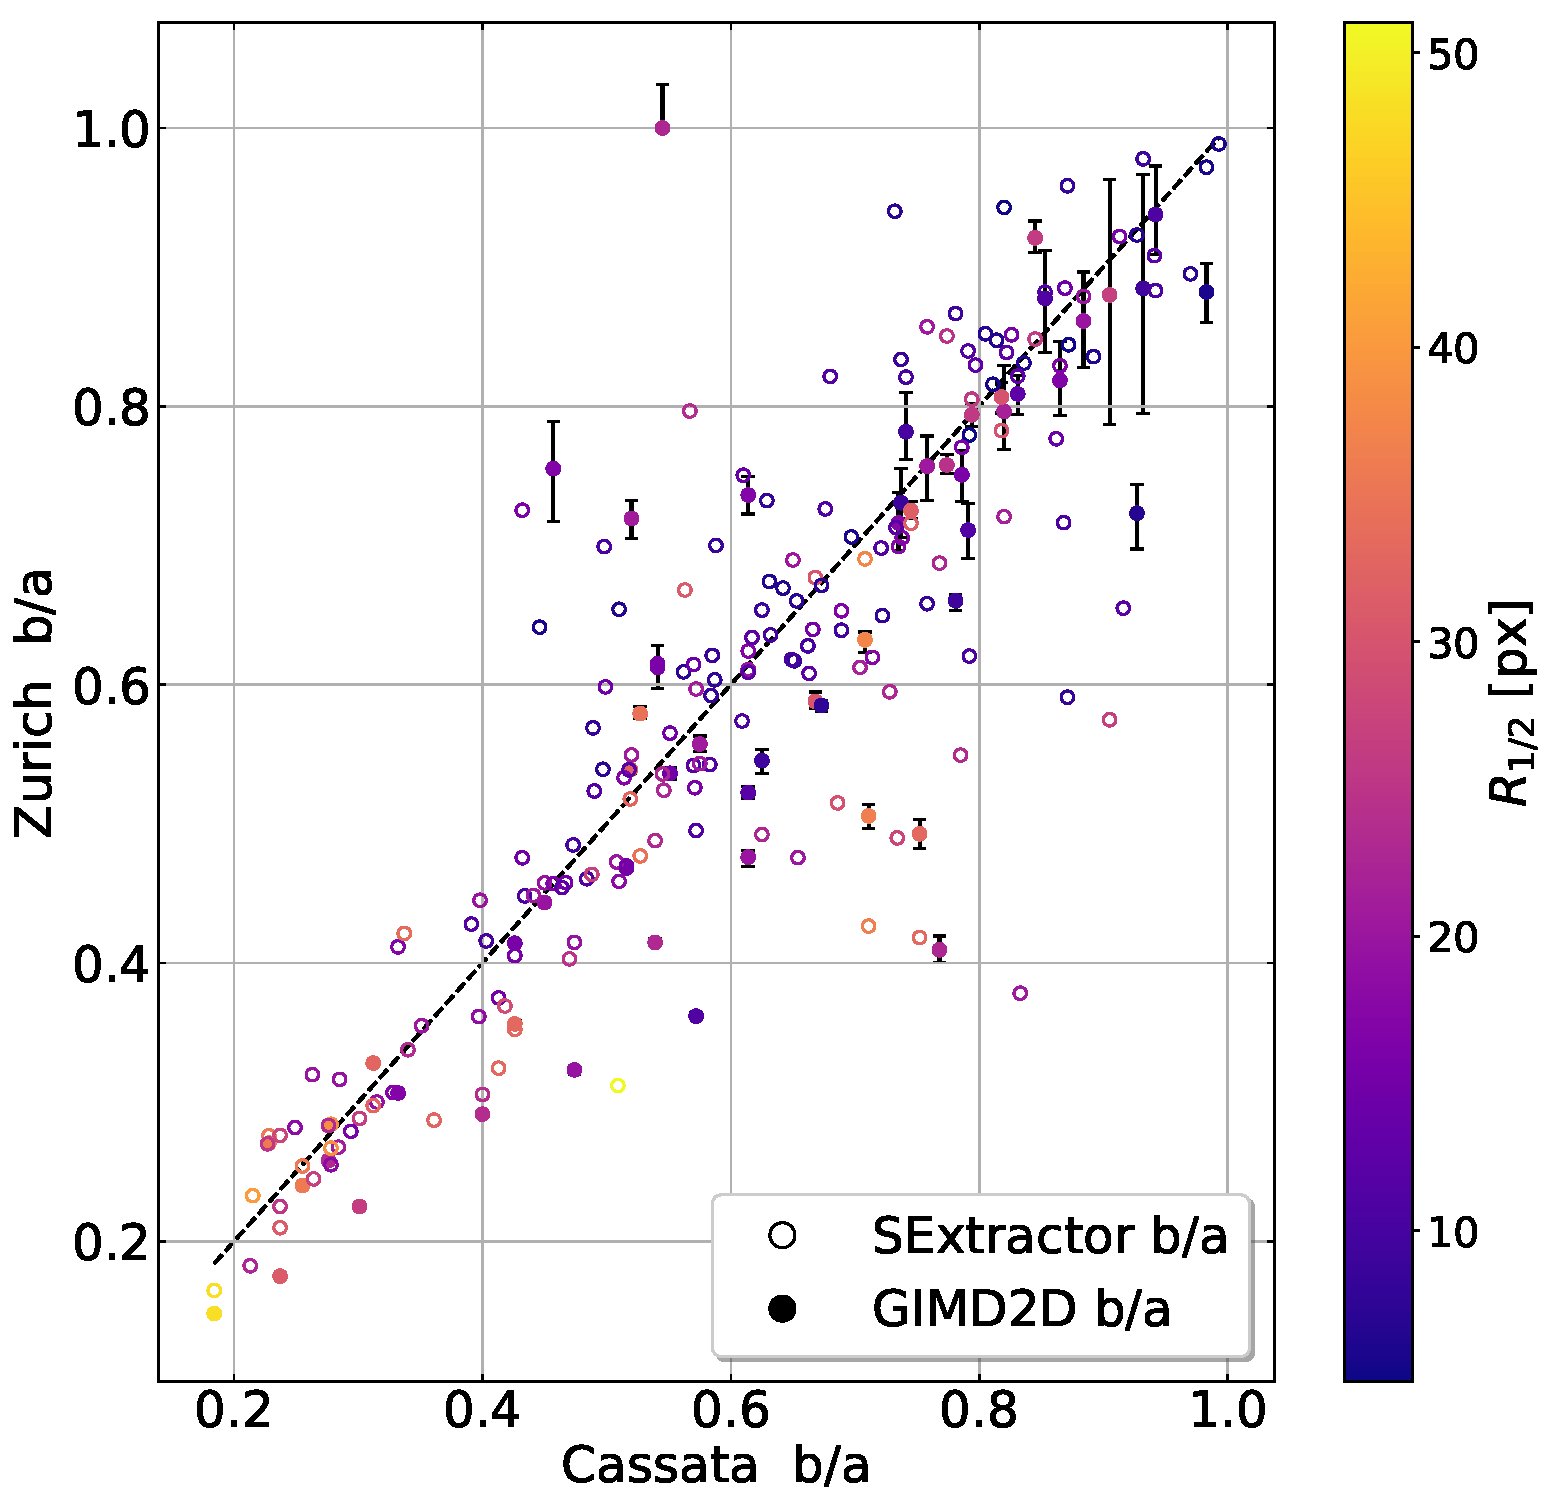
\includegraphics[width=\linewidth]{{../Plots/checkMorpho/check_b_a}.pdf}
		\subcaption{Axes ratio from Zurich and Cassata for the field galaxies. There is an overall good agreement between the catalogues and between Zurich and GIM2D. We find a similar dispersion for SExtractor and GIM2D of about $0.1$. No specific trend is found with the galaxies size.}
	\end{minipage}
	\hfill
	\begin{minipage}[c]{0.49\linewidth}
		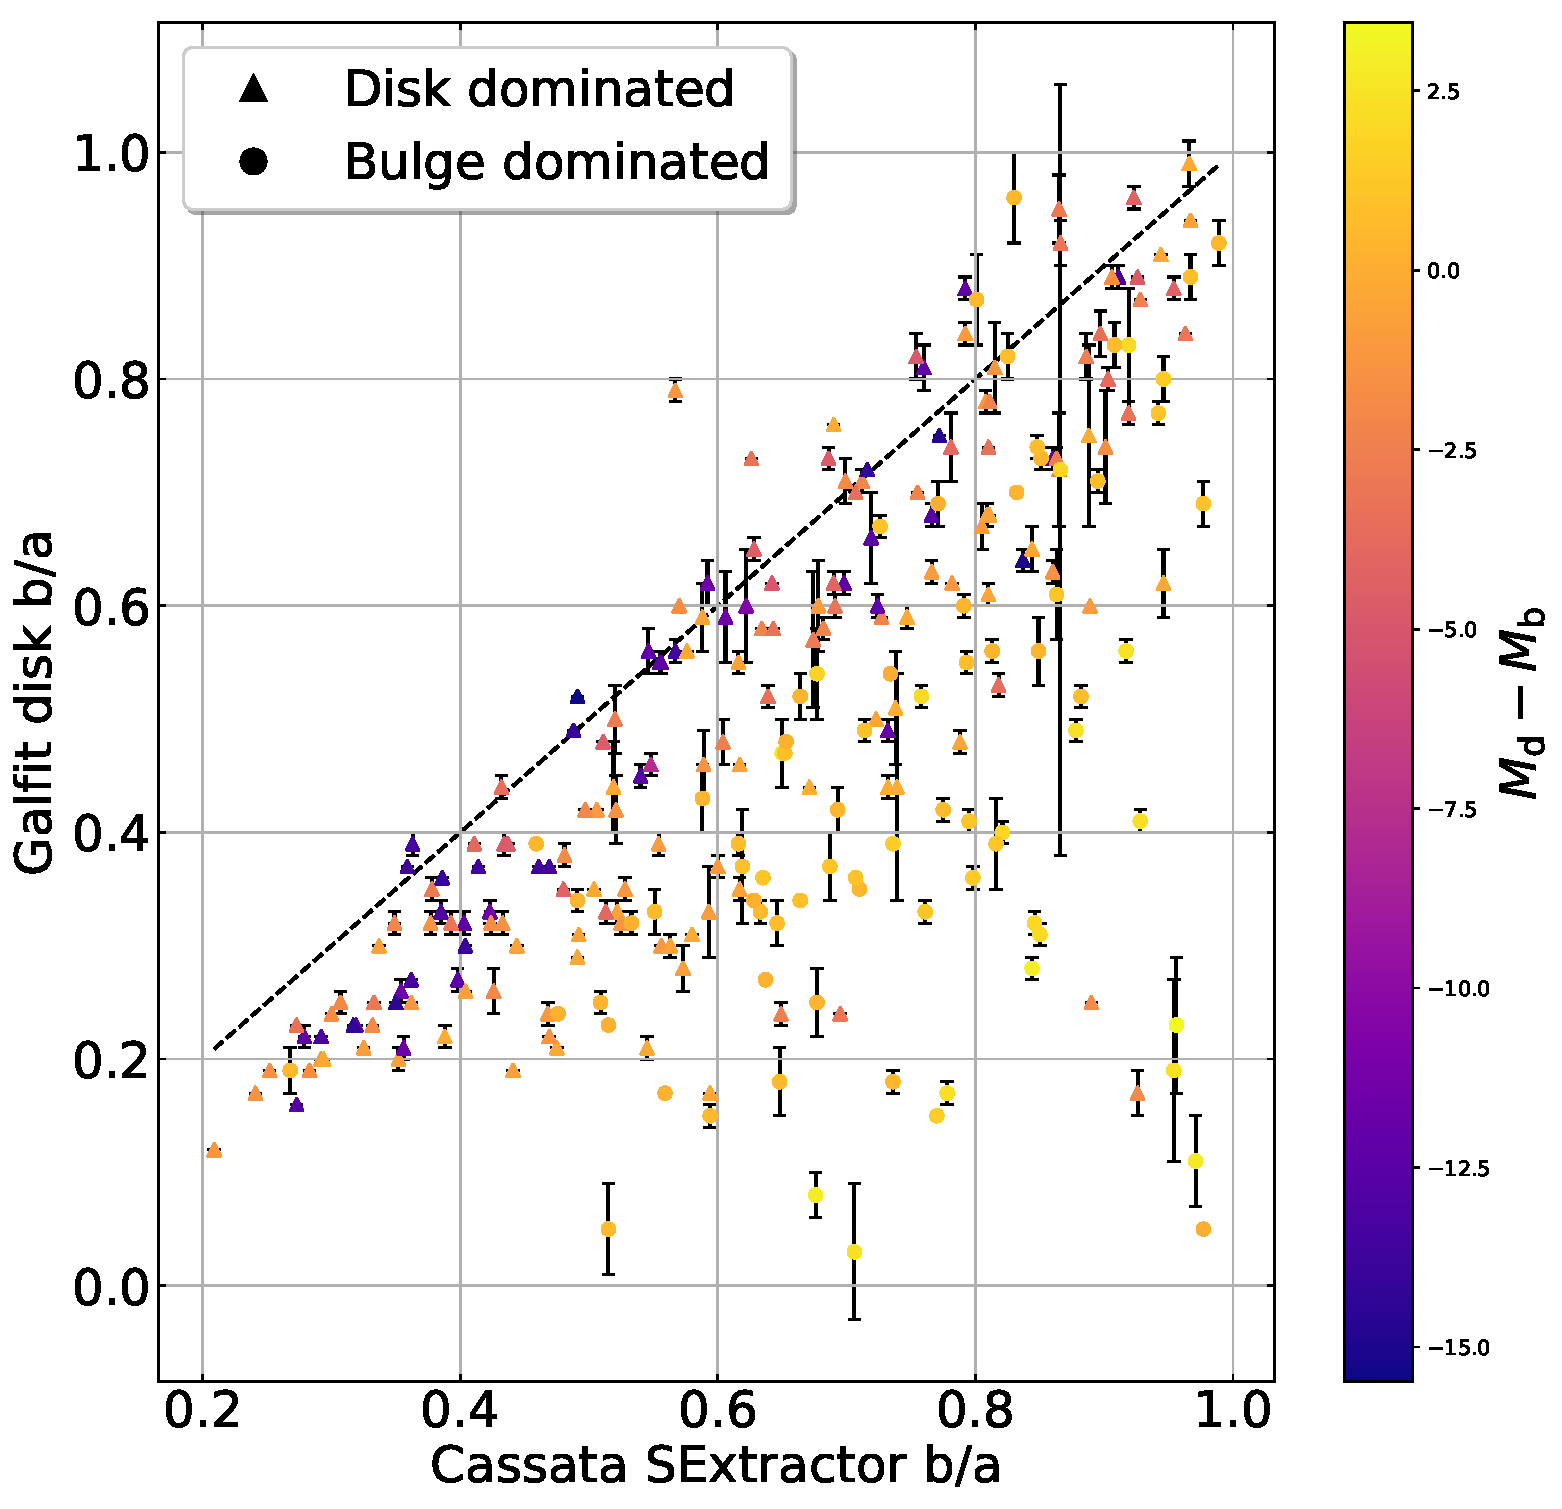
\includegraphics[width=\linewidth]{{../Plots/checkMorpho/check_b_a_GF}.pdf}
		\subcaption{GALFIT axes ratio against that of Cassata for galaxies in structures. Globally, the axes ratio in the catalogue seems to be underestimated. If we separate the galaxies as disk or bulge dominated according to the most luminous component, we find that most of the scatter comes from elliptical galaxies.}
	\end{minipage}
	\caption[Ellipticity robustness]{Comparison between Cassata, Zurich and GALFIT $b/a$ axes ratio. Zurich catalogue gives two values computed with SExtractor and GIM2D, and Cassata only with SExtractor. Error bars are only available for a few GIM2D and GALFIT values.}
	\label{fig:check_ellipticity}
\end{figure}

As mentioned in previous sections, the ellipticity is a critical parameter which is used to compute a value for the inclination of the galaxies. It is related to the $b/a$ ratio given in the catalogues, so we can compare it as a proxy for the ellipticity. This is illustrated in Fig.\,\ref{fig:check_ellipticity} 
\begin{enumerate*}[label={(\alph*)}]
	\item where the axes ratio is compared for field galaxies for which we could assign a radius as described in Section \ref{sec:comp_radii}. In Fig.\,\ref{fig:check_ellipticity}
	\item where GALFIT $b/a$ is compared with that of Cassata for galaxies in structures.
\end{enumerate*}
Catalogues give consistent values for field galaxies with most of the scatter coming from the region where $0.4 < b/a < 0.8$. We checked that the size of the galaxies did not impact too much on the error, but we did not find any specific trend. We also checked that catalogues values are comparable to that of GALFIT. In this case, we find a large scatter with the catalogues axes ratio underestimated with respect to GALFIT value for almost all galaxies. Since GALFIT fits two components on the light profile, we expect the galaxies with a dominant bulge to have a less constrained $b/a$ ratio. To check this effect, we colour coded the points according to the difference in magnitude between GALFIT disk and bulge components $M_{\rm{d}}^{\rm{GF}} - M_{\rm{b}}^{\rm{GF}}$. We observe that the majority of the scatter actually comes from bulge dominated galaxies, i.e. ellipticals, for which $M_{\rm{d}}^{\rm{GF}} - M_{\rm{b}}^{\rm{GF}} > 0$.














\newpage
\subsection{SNR and size selection}
\label{sec:cut}

\subsubsection{Size selection}
\label{sec:cut_size}

The first parameter we can think of to make our selection is the size of the galaxies. We already checked in Section\,\ref{sec:comp_radii} biases which might arise, investigated their origins, and corrected them. Now that we have reliable values, we need to define a selection criterion. Based on \shortciteA{Bacon2015} and \shortciteA{Bacon2017}, the MUSE Point Spread Function (PSF), that is the pattern we obtain when we observe a point-like source with MUSE, can either be described by   a \shortciteA{MoffatProfile} or a Gaussian profile. In practice, they showed that a Gaussian best fits the PSF for MUSE images, so we used this profile in the following parts whenever we needed an estimate of the PSF. \\

The PSF Full Width at Half Maximum ($\rm{FWHM}$) is directly related to the seeing conditions, and it can be easily derived from the relation $I_{\rm{PSF}} ( \rm{FWHM}/2) = I_0 /2$. Since it gives us information about the minimum spatial extent within which we start to loose information, we could use it as a starting point for our selection criterion. Moreover, we will need a reliable measure of the PSF $\rm{FWHM}$ for each galaxy when performing the kinematical modelling. Indeed, according to the aforementioned articles the value of the $\rm{FWHM}$ is expected to linearly decrease with wavelength. All galaxies are observed via their [OII] $\lambda\lambda 3729, \SI{3729}{\angstrom}$ doublet at the same rest-frame wavelength. But, given that they are all located at a different redshift $z$, we actually observe them at wavelengths covering the entire MUSE spectrum, that is we have the usual relation $\lambda_{\rm{obs}} = \lambda_{\rm{em}} ( 1 + z )$, where $\lambda_{\rm{em}}$, $\lambda_{\rm{obs}}$ are the emitted (rest-frame) and observed wavelengths respectively. Therefore, there is not just one $\rm{FWHM}$ value per field, but one per galaxy. \\

To derive this value, we need to compute the linear evolution in each field by measuring the $\rm{FWHM}$ of stars for at least two different wavelengths. Assuming seeing conditions are similar within a field (no spatial dependence), we can use the same relation per MUSE field to compute the $\rm{FWHM}$ for the observed [OII] wavelength at the redshift of the galaxies. These measures had already been done by B. Epinat and V. Abril-Melgajero on at least two stars per field. Though a more rigorous modelling of the wavelength variation of the PSF $\rm{FWHM}$ including both more data points and potentially higher order terms is mandatory for future analysis, we decided to stick to these values in the present work, keeping in mind the uncertainties which will affect the velocity dispersion maps in the modelling section. A representation of the $\rm{FWHM}$ variation with wavelength for the 16 MUSE fields is shown in Fig.\,\ref{fig:FWHM_var_lambda}. Most MUSE fields have $\rm{FWHM}$ values below $\SI{0.7}{"}$ which is not surprising given that it was one of the constraints of the observations.\\

To have a criterion which is not galaxy dependent, we decided to keep galaxies with a size $2 R_{1/2} \geq \SI{0.7}{"}$ since this corresponds to an upper limit for the $\rm{FWHM}$ for almost every field. Moreover, according to \shortciteA{Swinbank2017} who compared the half-light radius of the nebular [OII] emission in MUSE images with that of their HST counterpart in ACS \textit{I} or WFC3 \textit{H}-band, the [OII] half-light radius seems to scale with the broad-band continuum HST radius as 

\begin{equation}
	R_{1/2}^{\rm{OII}} = (1.18 \pm 0.03) R_{1/2}^{\rm{HST}}
\end{equation}

Thus, by using an upper limit, we may loose a few galaxies which might have been resolved enough. Nevertheless, given the time constraints, this was mandatory if we wanted to keep a sample of reasonable size.



\subsubsection{SNR selection}
\label{sec:cut_SNR}

The other information we use to select our sample is the signal to noise ratio. The $\rm{SNR}$ is generally derived as the ratio between the source's signal and the background level. The noisier an image, the lower the SNR is. Given that galaxy pixels dominated by noise will be removed before the modelling by an automatic cleaning routine, we would like to keep galaxies with a high enough $\rm{SNR}$, so that there is still a significant amount of pixels useful for the analysis after the cleaning. In the MUSE pipeline, \textsc{PLATEFIT} \shortcite{Tremonti2004} was run on the integrated spectrum of the galaxies after deriving their redshift. This software uses a set of stellar spectra from \shortciteA{Bruzual2003} and \shortciteA{Sanchez2006} to fit and remove the continuum emission at the galaxy redshift. Each line is then fitted by a Gaussian profile individually with the same velocity offset and dispersion for all the lines. \textsc{PLATEFIT} returns galaxies spectral parameters such as the [OII] flux. From these, we used the flux and its error to compute a value for the $\rm{SNR}$

\begin{equation}
	\rm{SNR} = \frac{\rm{[OII] \,\, flux}}{\rm{[OII] \,\, flux \,\, error}}
\end{equation}

Since the typical $\rm{SNR}$ value used by the routine to remove noise dominated pixels in the MUSE maps is around $5$, we decided as a first step to choose an SNR lower limit of $10$ on the [OII] flux measured in integrated spectra, allowing us to keep galaxies with strong enough detection.


\newpage
\subsubsection{Inspecting galaxies}
\label{sec:selecting_galaxies}

We visually inspected galaxies around the $\rm{SNR}$ and the size cuts in order to quantify
\begin{enumerate*}[label={(\alph*)}]
	\item how many resolved galaxies would be lost if we applied the criteria given in Sec.\,\ref{sec:cut_size} and \ref{sec:cut_SNR} (false negative)
	\item how many unresolved galaxies would be selected in our sample (false positive).
\end{enumerate*}
To do so, we defined four boxes: $5 \leq \rm{SNR} \leq 10$, $10 \le \rm{SNR} \leq 15$, $0.25" \leq R_{1/2} \leq 0.35"$ and $0.35" \le R_{1/2} \leq 0.45"$ containing $46$, $20$, $58$ and $49$ galaxies respectively. The selected galaxies according to the criteria defined in Sections \ref{sec:cut_size} and \ref{sec:cut_SNR}, as well as the the cuts and the boxes are represented in Fig.\,\ref{fig:sample_selection} \\

\begin{wrapfigure}{l}{.58\linewidth}
	\centering
	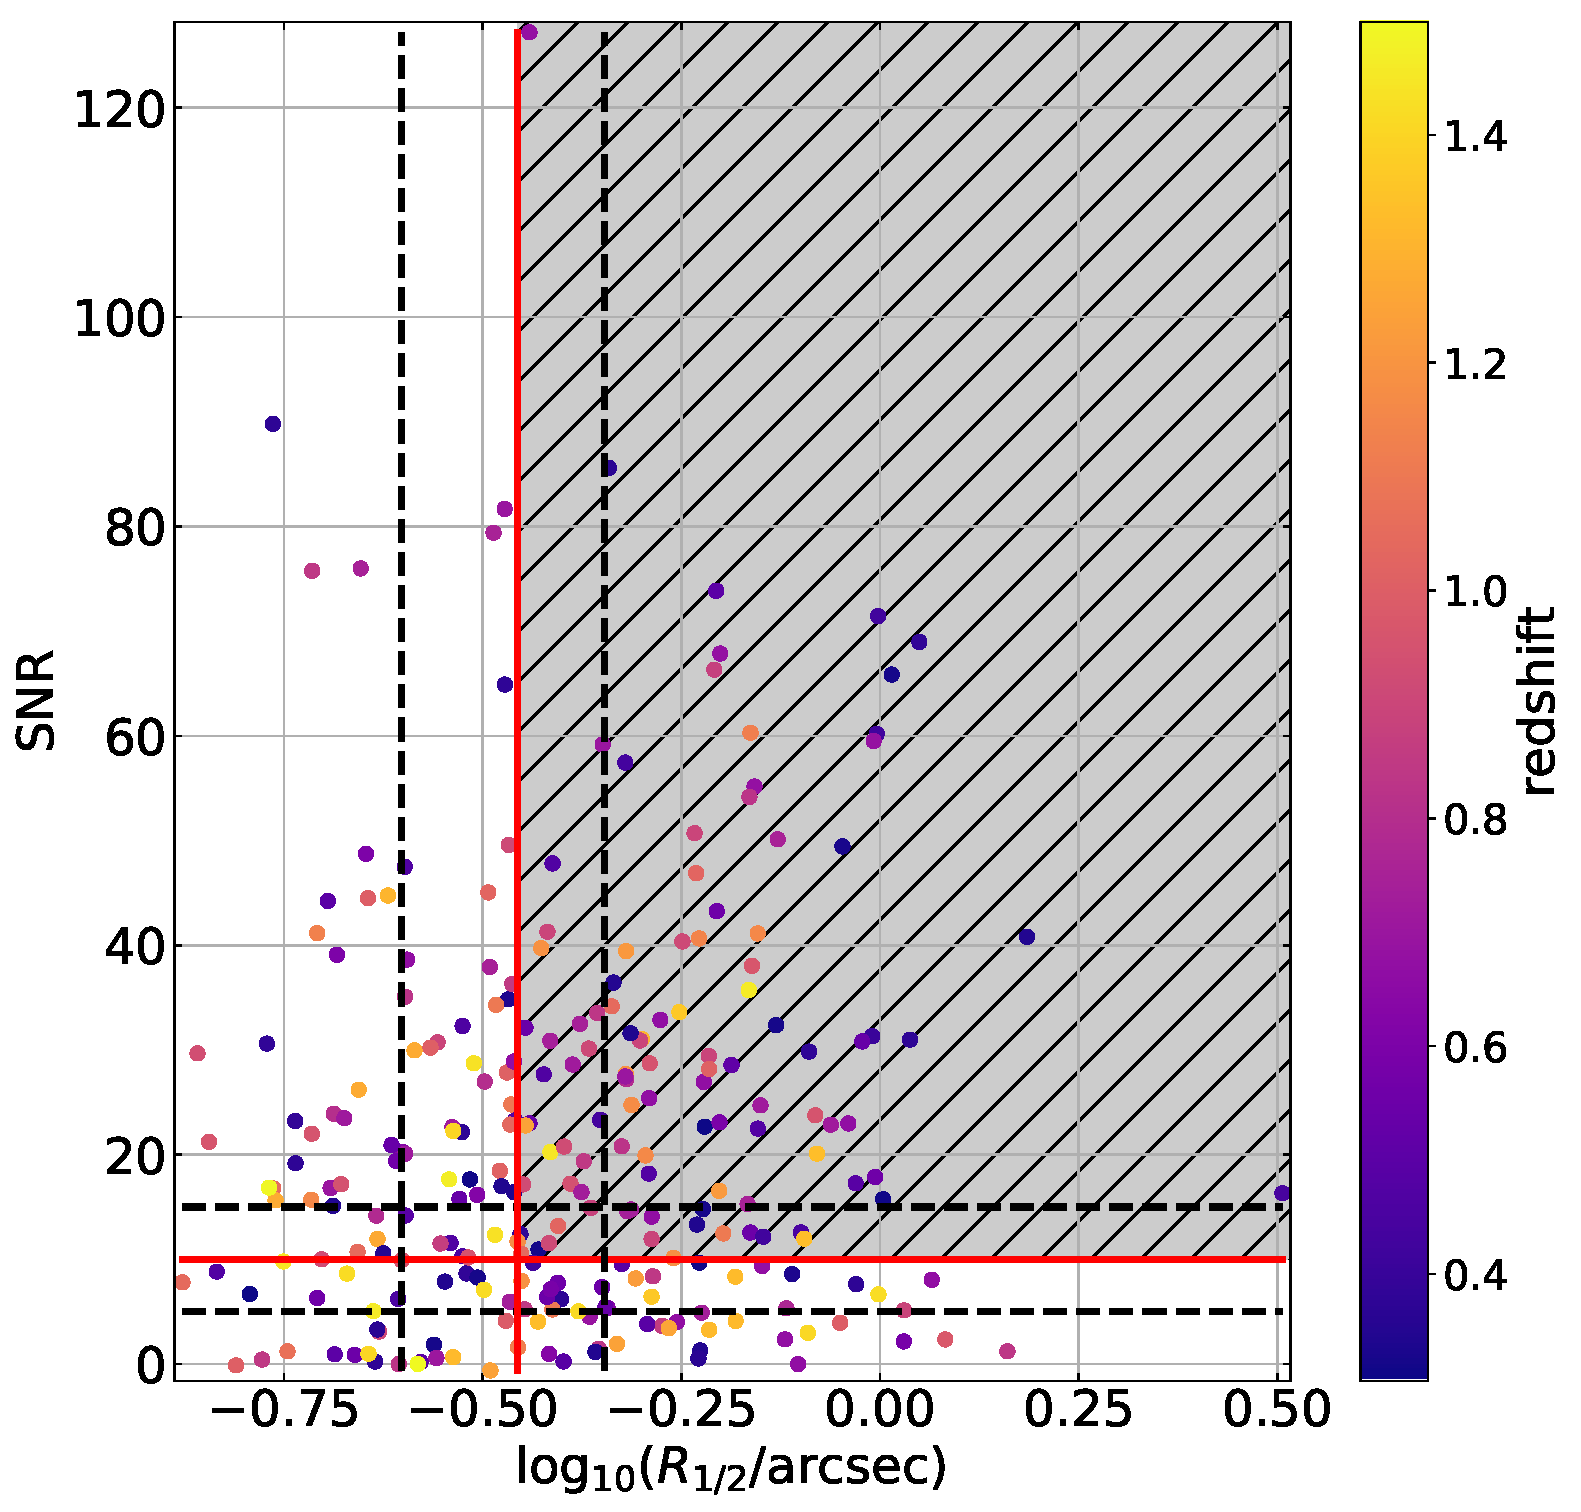
\includegraphics[width=\linewidth]{{../Plots/Selection_plots/SNR_vs_R_halfLight_arcsec}.pdf}
	\caption[Sample selection]{Full sample of $261$ field galaxies with our selection box over-plotted (hatched area). Galaxies with $5 \leq \rm{SNR} \leq 15$ and $0.25" \leq R_{1/2} \leq 0.45"$ (bounds plotted as dashed lines) were visually inspected to check how many resolved galaxies we might have lost. Selection criteria from Sec.\,\ref{sec:cut} are also plotted as solid red lines. No specific trend appear with redshift.}
	\label{fig:sample_selection}
\end{wrapfigure}

We then ran an automatic cleaning routine for all the decided togalaxies in these boxes. The algorithm used removes any pixel which either has its $\rm{SNR}$ below $5$ or a dispersion below a certain percentage $\gamma$ of the velocity dispersion $\sigma_{\rm{v}}$ computed from the Line Spread Function (LSF) $\rm{FWHM}$. The LSF corresponds to the spectral equivalent of a spatial PSF, and tells us how much the instrument will broaden out an infinitely thin line. According to \shortcite{Bacon2017} and \shortcite{Guerou2017} who measured the LSF variation with wavelength in the Hubble Ultra Deep Field (HUDF) and Hubble Deep Field South (HDFS) and who found that it was stable through time, we computed the LSF $\rm{FWHM}$ as

\begin{equation}
	\rm{FWHM} = a \lambda^2 + b \lambda + c
\end{equation}
with $a = 5.866 \times 10^{-8}$, $b = - 9.187 \times 10^{-4}$, $c = 6.040$. The $\rm{FWHM}$ and $\lambda$ (observed wavelength) are in angstroms. Thus, the LSF $\rm{FWHM}$ will depend upon the redshift of the galaxy as well. It is related to the velocity dispersion via

\begin{equation}
	\frac{\sigma_{\rm{v}}}{c} = \frac{\sigma}{\lambda_{\rm{em}} (1+z)}
\end{equation}
where $\sigma = \rm{FWHM} \left (2 \sqrt{2 \log 2} \right )^{-1}$ is the spectral dispersion due to the LSF. \\

The choice to keep pixels with a velocity dispersion above $\gamma \sigma_{\rm{v}}$ was motivated by the fact that sky lines from OH molecules in the atmosphere can generate fake emission lines, mimicking the [OII] doublet. Sky subtraction during the data reduction can indeed produce fake residuals with P-cygni profiles for the brightest OH sky lines in the MUSE datacubes. However, these are always found to have a width below the LSF $\rm{FWHM}$. So any pixel with a fake detection will be removed with this criterion. The percentage $\gamma$, which we chose to be $80\%$, is meant to not remove pixels with real detection which might have thin lines.\\

After visually inspecting the galaxy sizes in the cleaned [OII] maps, we classified them as resolved if they had a large enough extension (typically larger than the PSF $\rm{FWHM}$) or not otherwise. Among the $261$ field galaxies which have morphological information in the catalogues, $103$ fall into the limits imposed in Sec.\,\ref{sec:cut}. We find that roughly $26\%$ of the galaxies below the cuts are actually false negatives and that $15\%$ above them are false positives. Since this classification is purely visual, slightly relaxing the constraints on to whether a galaxy is resolved enough or not allow these values to vary by roughly $10\%$. Our criteria for the selection therefore seem reasonable, though in future works we might increase our sample by a factor of $\sim 1.5$ by visually inspecting each galaxy separately.





\newpage
\subsection{Characterisation of the sample}
\label{sec:sample_characterisation}

\subsubsection{Redshift distribution}

\begin{wrapfigure}{r}{.4\linewidth}
	\centering
	\vspace{10pt}
	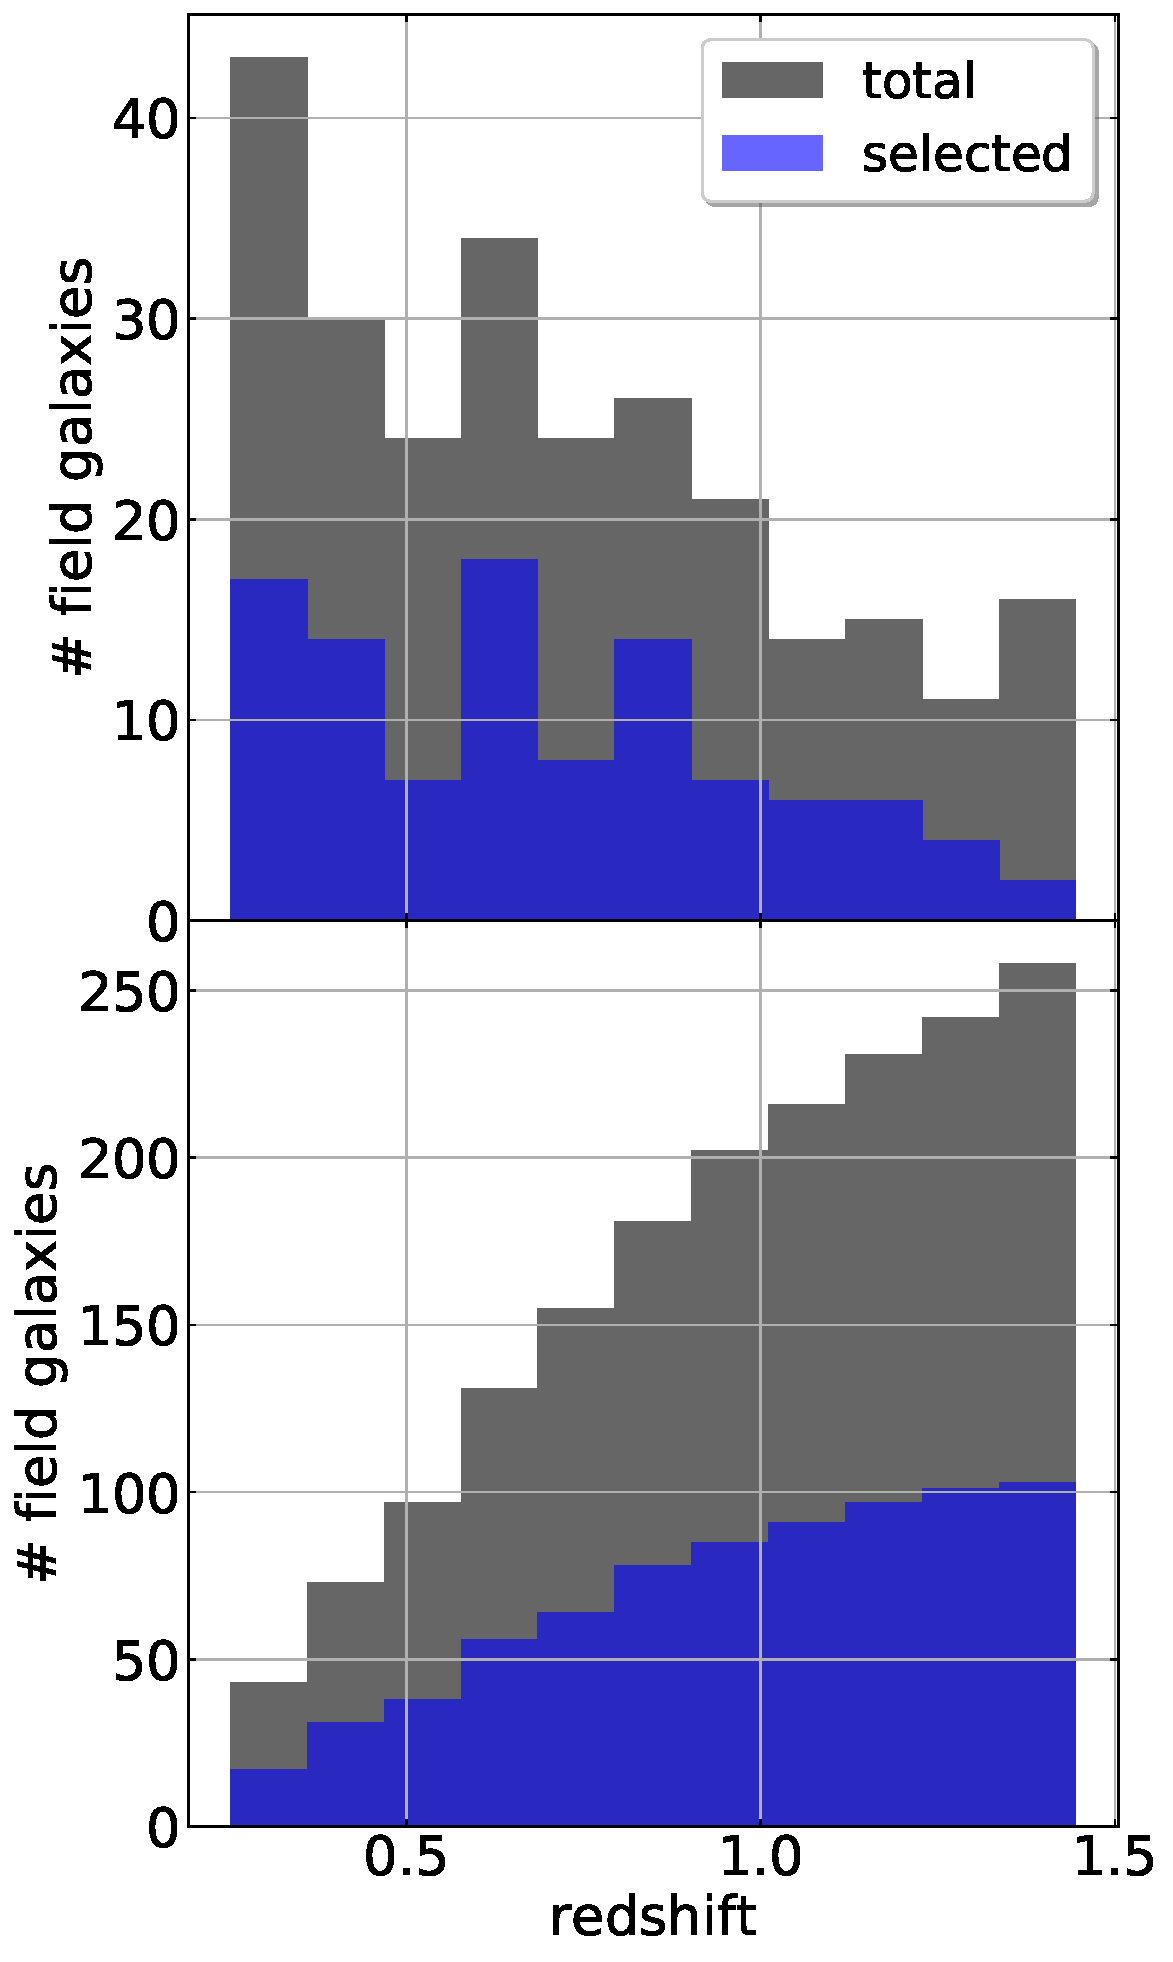
\includegraphics[width=\linewidth]{{../Plots/Selection_plots/cumulative_hist_redshift}.pdf}
	\caption[Redshift distribution]{Redshift distribution of the total sample (grey) and selected (blue) galaxies. Redshift bins of size $0.1$ have been used. Top: density plot as a function of redshift. Bottom: cumulative distribution. We lack most of the galaxies at redshift $1.4$. The redshift distribution of the selcted galaxies remains consistent with the original one.}
	\label{fig:redshift_distribution}
\end{wrapfigure}

The choice of the [OII] $\lambda\lambda 3729, \SI{3729}{\angstrom}$ doublet for the kinematical analysis was mainly due to the large range of redshift it covers given the MUSE spectral range. We therefore had in our catalogue galaxies spanning a redshift domain from $0.3$ to about $1.4$. As shown in Fig.\,\ref{fig:redshift_distribution}, we loose after our selection a significant fraction of galaxies at all redshifts, and in particular the majority of the most distant galaxies. It is not surprising to loose galaxies at high redshift as these have the lowest angular sizes on the sky at a fixed physical length. Nevertheless, we are globally selecting more galaxies per redshift bin than we are putting aside. The average and median redshifts are $0.749$ and $0.719$ for the selected galaxies, $0.809$ and $0.750$ for the unselected ones. Thus, our sample remains consistent in terms of redshift even after the selection.



%\newpage
\subsubsection{Mass-SFR relation}

Our sample spans 3 orders of magnitude both in mass and $\rm{SFR}$ in the ranges $10^{8.07} \leq M / \si{M_{\odot}} \leq  10^{11.1}$ and $0.04 \leq \rm{SFR} / ( \si{M_{\odot}. yr^{-1} }) \leq 126$. We investigate our sample in the mass-$\rm{SFR}$ diagram in Fig.\,\ref{fig:sfr_vs_mass}. Star-forming galaxies are expected to lie on a diagonal line $\log M$-$\log \rm{SFR}$ space, with some scatter, called the galaxies Main Sequence (MS). A few highly star-forming galaxies such as starburst galaxies and Ultra Luminous InfraRed Galaxies (ULIRG/LIRG) are generally found above the main sequence. Massive quiescent (low $\rm{SFR}$) galaxies can also be found below the MS. In our sample, we recover galaxies on the main-sequence after the selection. We loose massive galaxies with low SFR which is probably due to the fact that we are selecting galaxies with a high enough [OII] surface brightness. Since [OII] flux comes from ionised regions which correlate with star formation, most quiescent galaxies are eliminated during observation, and the few large enough to be detected will have too low $\rm{SNR}$ values to be selected. We also loose the very low mass end of our sample ($\log_{10} (M / \rm{M_{\odot}}) \lesssim 8.5$). This is explained by the fact that there exists a scaling relation between a galaxy mass and its radius so that more massive galaxies are also larger and vice-versa. Thus, it appears that the very low mass end is removed from our sample when performing the size selection. \\

\begin{wrapfigure}{l}{0.5\linewidth}
	\centering
	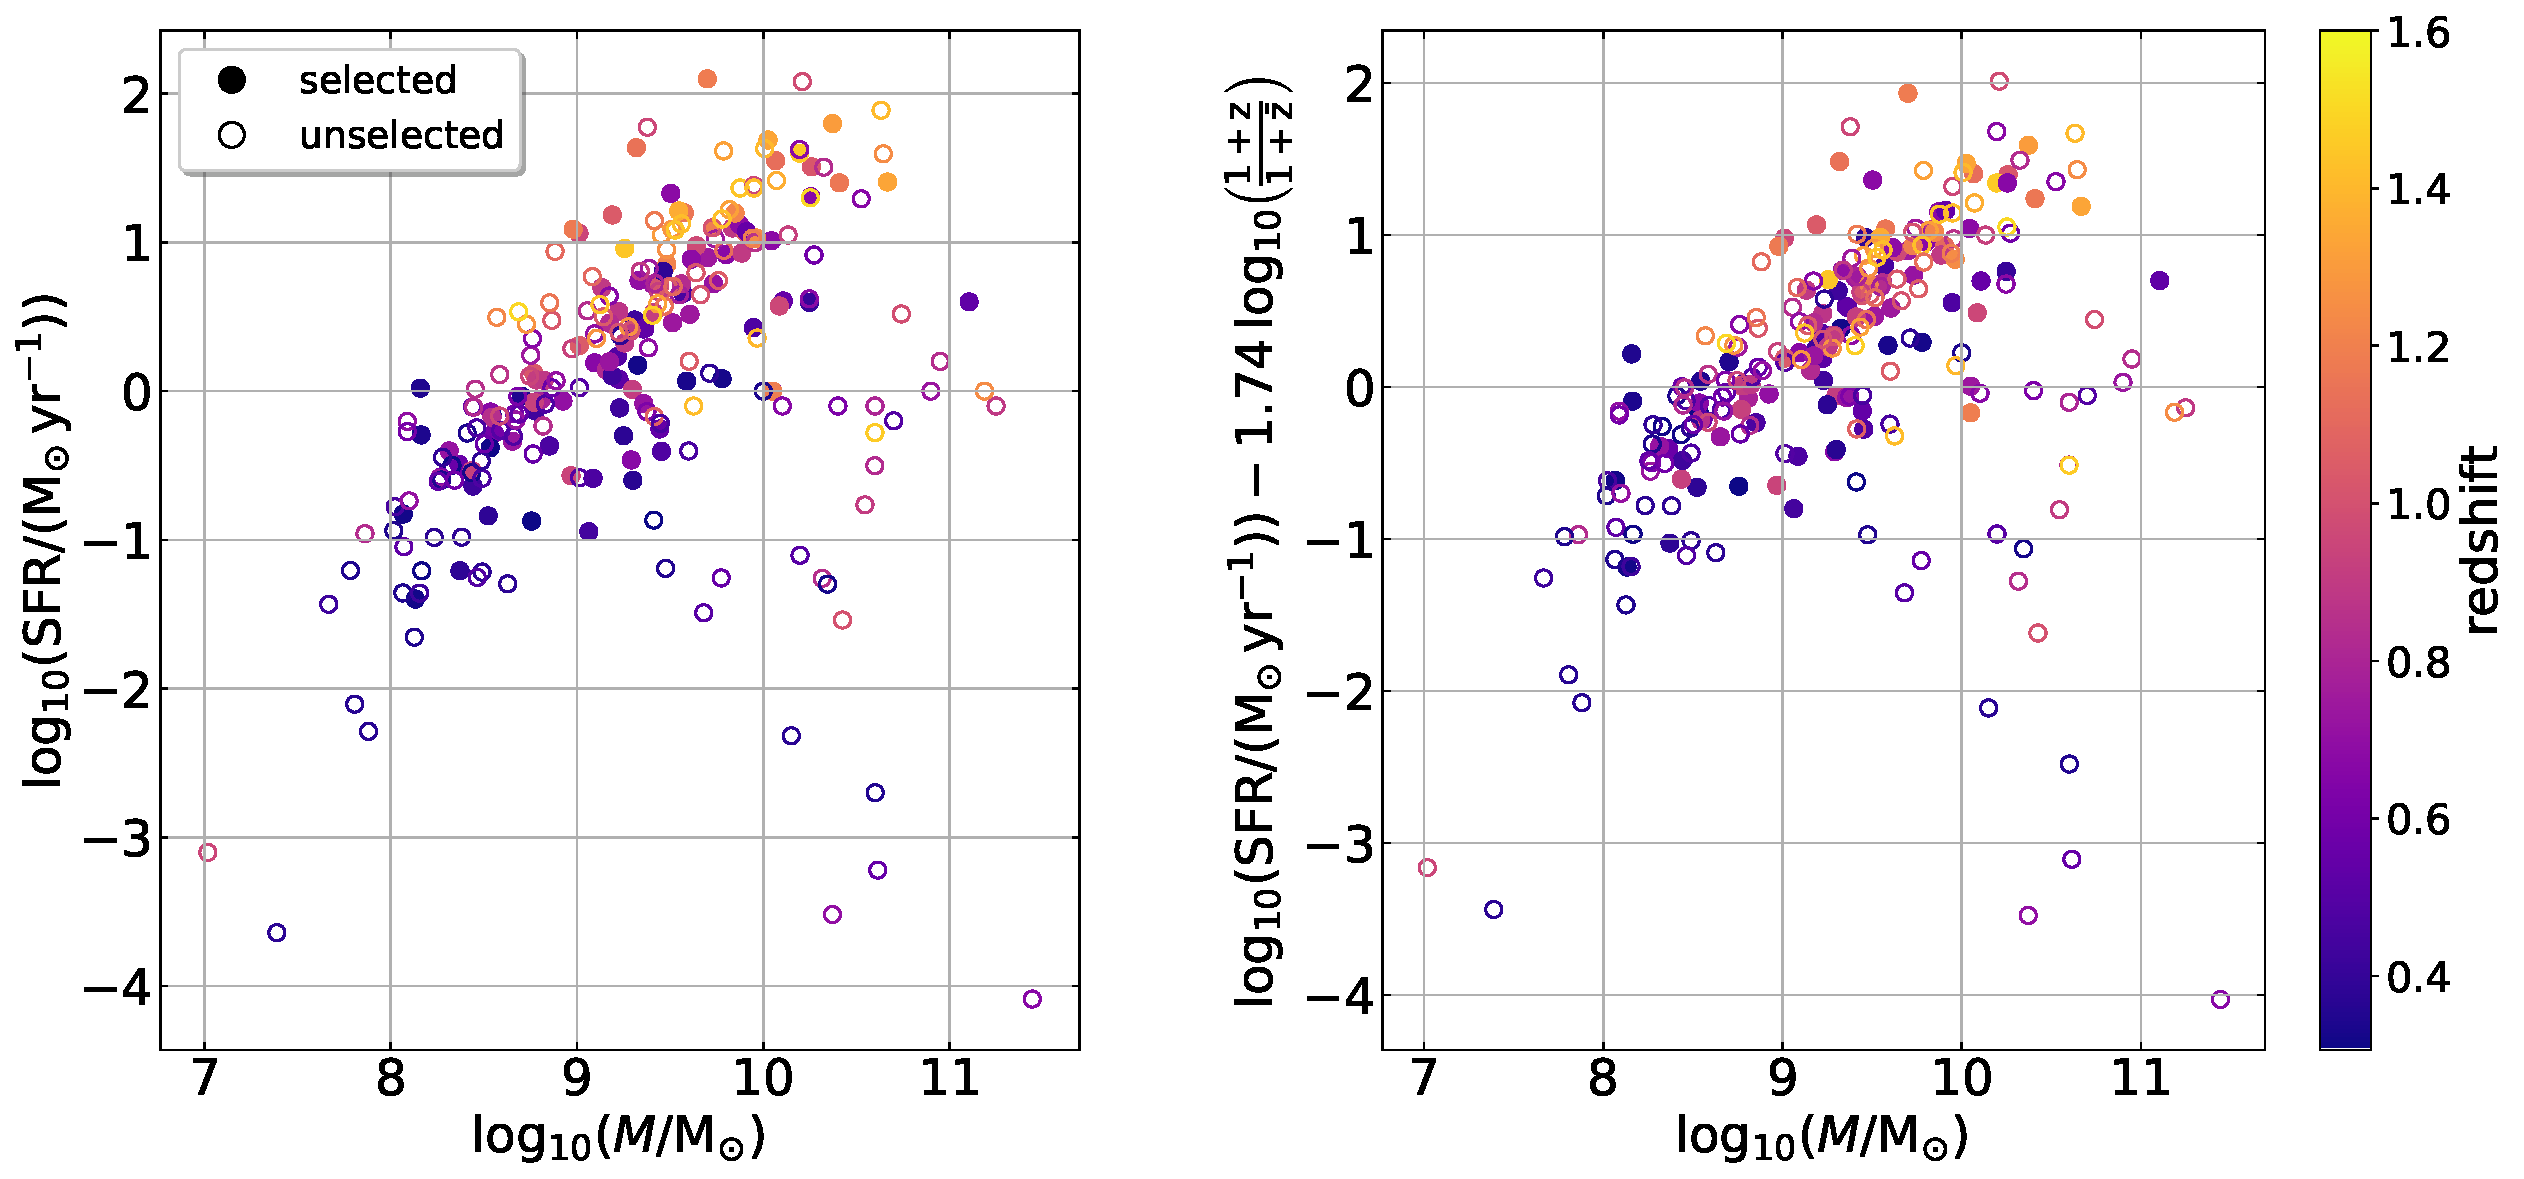
\includegraphics[width=\linewidth]{{../Plots/Selection_plots/SFR_vs_mass_withoutFAST}.pdf}
	\caption[SFR-mass relation]{SFR-mass relation for selected (filled circles) and unselected (open circles) galaxies. Left: SFR extracted from SED fitting \shortcite{laigle_cosmos2015_2016}. Right: the redshift corrected SFR as given in Eq.\,\ref{eq:SFR_corrected_redshift}. Most of our sample lies on the galaxies main sequence. We are loosing almost every massive quiescent galaxies on the lower right part of the plane, as well as the very low mass ones on the lower left.}
	\label{fig:sfr_vs_mass}
\end{wrapfigure}

We also took into account the redshift evolution of the main sequence. We refer to \shortciteA{Boogaard2018} who derived a this evolution for galaxies observed with MUSE in the HUDF on the main-sequence found roughly in the same redshift, mass and $\rm{SFR}$ intervals. They modelled the log of the $\rm{SFR}$ as a plane in $\log M - \log (1 + z)$ space

\begin{equation}
	\begin{split}
		\log_{10} \left ( \frac{\rm{SFR}}{\si{M_{\odot} . yr^{-1}}} \right ) & =  0.83_{-0.06}^{+0.07} \log_{10} \left ( \frac{M}{\si{M_{\odot}}} \right ) \\
		& - 0.83^{+0.05}_{-0.05} \\
		& + 1.74_{-0.68}^{+0.66} \log_{10} \left ( \frac{1+z}{1+z_0} \right )
	\end{split}
	\label{eq:SFR_corrected_redshift}
\end{equation}

where $z_0$ acts as a normalisation factor which will scale the relation at this redshift. We chose the median redshift of the selected galaxies to apply the $\rm{SFR}$ correction shown in Fig.\,\ref{fig:sfr_vs_mass}.


\clearpage
\subsubsection{Morphological type}
\label{morpho_type_classification}

\begin{wrapfigure}{l}{0.5\linewidth}

	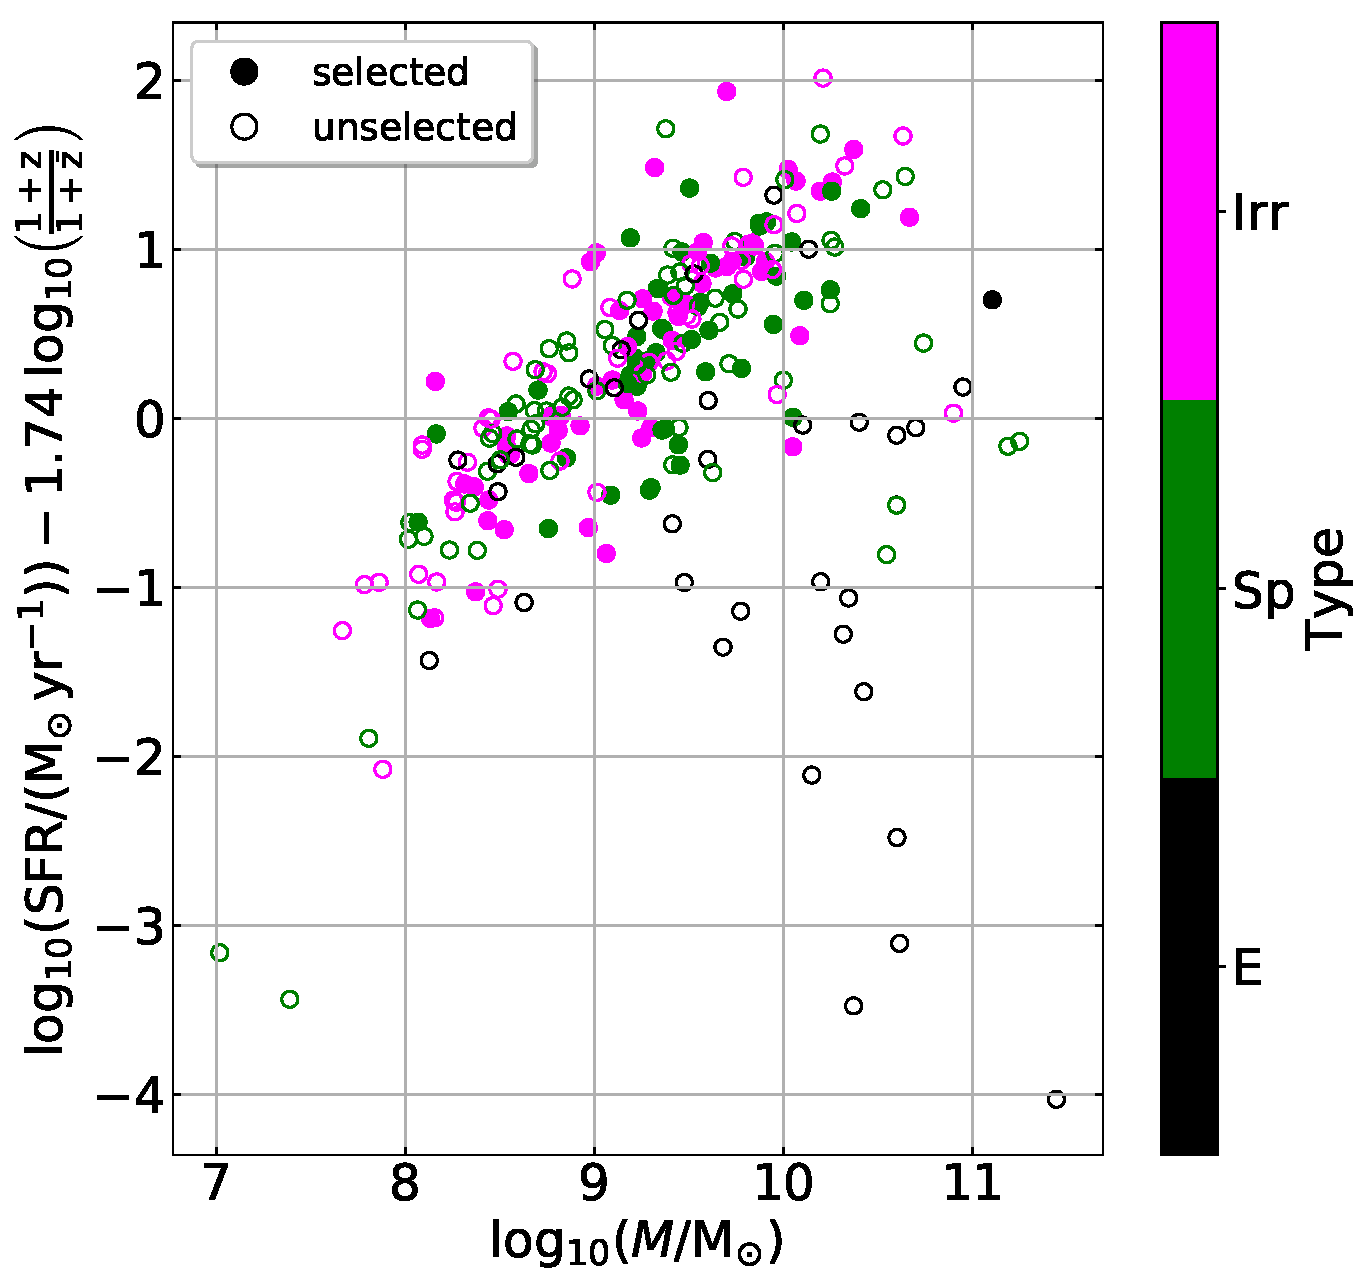
\includegraphics[width=\linewidth]{{../Plots/Selection_plots/SFR_vs_mass_morphoType}.pdf}
	\caption[Morphological types of the sample galaxies]{Mass-$\rm{SFR}$ diagram similar to Fig\,\ref{fig:sfr_vs_mass} colour coded according to the galaxies morphological classification. Massive quenched galaxies are all found to be classified as spheroidal systems. After the selection, we only recover irregular and disk-like galaxies, except for one massive star-forming spheroidal galaxy.}
	\label{fig:sfr-mass_morphoCoded}
\end{wrapfigure}

\begin{wrapfigure}{l}{0.5\linewidth}

	\includegraphics[width=\linewidth]{{Plots/inclination_distribution}.pdf}
	\caption[Selected galaxies inclination distribution]{Distribution of the inclination of the selected galaxies (blue) and of the total sample of galaxies with morphological parameters from HST catalogues (grey). }
	\label{fig:inc_distribution}
\end{wrapfigure}

To end the characterisation of our sample, we look at which galaxies are selected in terms of morphological type. This is illustrated in Fig.\,\ref{fig:sfr-mass_morphoCoded} where we used Cassata classification to separate galaxies. \\

We see that the massive quenched galaxies we are not selecting actually are spheroidal systems. Surprisingly enough, we loose every spheroidal galaxy (except one), in particular those found on the main-sequence. In the end, we mainly recover irregularly shaped galaxies and a significant fraction of disk-like galaxies as well.

\subsubsection{Inclination of the galaxies}






 
